\providecommand{\slides}{
  \newcommand{\slideshead}{
  \newcommand{\thepage}{\arabic{mypage}}
  %beamer
  \documentclass[t,hyperref={bookmarks=true}]{beamer}
%  \documentclass[t,hyperref={bookmarks=true},aspectratio=169]{beamer}
  \setbeamersize{text margin left=5mm}
  \setbeamersize{text margin right=5mm}
  \usetheme{default}
  \usefonttheme[onlymath]{serif}
  \setbeamertemplate{navigation symbols}{}
  \setbeamertemplate{itemize items}{{\color{black}$\bullet$}}

  \newwrite\keyfile

  %\usepackage{palatino}
  \stdpackages
  \usepackage{multimedia}

  %%% geometry/spacing issues
  %
  \definecolor{bluecol}{rgb}{0,0,.5}
  \definecolor{greencol}{rgb}{0,.6,0}
  %\renewcommand{\baselinestretch}{1.1}
  \renewcommand{\arraystretch}{1.2}
  \columnsep 0mm

  \columnseprule 0pt
  \parindent 0ex
  \parskip 0ex
  %\setlength{\itemparsep}{3ex}
  %\renewcommand{\labelitemi}{\rule[3pt]{10pt}{10pt}~}
  %\renewcommand{\labelenumi}{\textbf{(\arabic{enumi})}}
  \newcommand{\headerfont}{\helvetica{13}{1.5}{b}{n}}
  \newcommand{\slidefont} {\helvetica{10}{1.4}{m}{n}}
  \newcommand{\codefont} {\helvetica{8}{1.2}{m}{n}}
  \renewcommand{\small} {\helvetica{9}{1.4}{m}{n}}
  \renewcommand{\tiny} {\helvetica{8}{1.3}{m}{n}}
  \newcommand{\ttiny} {\helvetica{7}{1.3}{m}{n}}

  %%% count pages properly and put the page number in bottom right
  %
  \newcounter{mypage}
  \newcommand{\incpage}{\addtocounter{mypage}{1}\setcounter{page}{\arabic{mypage}}}
  \setcounter{mypage}{0}
  \resetcounteronoverlays{page}

  \pagestyle{fancy}
  %\setlength{\headsep}{10mm}
  %\addtolength{\footheight}{15mm}
  \renewcommand{\headrulewidth}{0pt} %1pt}
  \renewcommand{\footrulewidth}{0pt} %.5pt}
  \cfoot{}
  \rhead{}
  \lhead{}
%  \rfoot{{\tiny\textsf{AI -- \topic -- \subtopic -- \arabic{mypage}/\pageref{lastpage}}}}
%  \rfoot{\vspace*{-4.5mm}{\tiny\textsf{\topic\ -- \subtopic\ -- \arabic{mypage}/\pageref{lastpage}}}\hspace*{-4mm}}
  \rfoot{\vspace*{-4.5mm}{\tiny\textsf{\color{gray}\topic\ -- \subtopic\ -- \arabic{mypage}/\pageref{lastpage}}}\hspace*{-4mm}}
  %\lfoot{\raisebox{5mm}{\tiny\textsf{\slideauthor}}}
  %\rfoot{\raisebox{5mm}{\tiny\textsf{\slidevenue{} -- \arabic{mypage}/\pageref{lastpage}}}}
  %\rfoot{~\anchor{30,12}{\tiny\textsf{\thepage/\pageref{lastpage}}}}
  %\lfoot{\small\textsf{Marc Toussaint}}

  \definecolor{grey}{rgb}{.8,.8,.8}
  \definecolor{head}{rgb}{.85,.9,.9}
  \definecolor{blue}{rgb}{.0,.0,.5}
  \definecolor{green}{rgb}{.0,.5,.0}
  \definecolor{red}{rgb}{.8,.0,.0}
  \newcommand{\inverted}{
    \definecolor{main}{rgb}{1,1,1}
    \color{main}
    \pagecolor[rgb]{.3,.3,.3}
  }
  %auto-ignore
  \renewcommand{\a}{\alpha}
  \renewcommand{\b}{\beta}
  \renewcommand{\d}{\delta}
    \newcommand{\D}{\Delta}
    \newcommand{\e}{\epsilon}
    \newcommand{\g}{\gamma}
    \newcommand{\G}{\Gamma}
  \renewcommand{\l}{\lambda}
  \renewcommand{\L}{\Lambda}
    \newcommand{\m}{\mu}
    \newcommand{\n}{\nu}
    \newcommand{\N}{\nabla}
  \renewcommand{\k}{\kappa}
  \renewcommand{\o}{\omega}
  \renewcommand{\O}{\Omega}
    \newcommand{\p}{\phi}
    \newcommand{\ph}{\varphi}
  \renewcommand{\P}{\Phi}
  \renewcommand{\r}{\varrho}
    \newcommand{\s}{\sigma}
  \renewcommand{\S}{\Sigma}
  \renewcommand{\t}{\theta}
    \newcommand{\T}{\Theta}
  %\renewcommand{\v}{\vartheta}
    \newcommand{\x}{\xi}
    \newcommand{\X}{\Xi}
    \newcommand{\Y}{\Upsilon}
    \newcommand{\z}{\zeta}

  \renewcommand{\AA}{{\cal A}}
    \newcommand{\BB}{{\cal B}}
    \newcommand{\CC}{{\cal C}}
    \newcommand{\cc}{{\cal c}}
    \newcommand{\DD}{{\cal D}}
    \newcommand{\EE}{{\cal E}}
    \newcommand{\FF}{{\cal F}}
    \newcommand{\GG}{{\cal G}}
    \newcommand{\HH}{{\cal H}}
    \newcommand{\II}{{\cal I}}
    \newcommand{\KK}{{\cal K}}
    \newcommand{\LL}{{\cal L}}
    \newcommand{\MM}{{\cal M}}
    \newcommand{\NN}{{\cal N}}
    \newcommand{\oNN}{\overline\NN}
    \newcommand{\OO}{{\cal O}}
    \newcommand{\PP}{{\cal P}}
    \newcommand{\QQ}{{\cal Q}}
    \newcommand{\RR}{{\cal R}}
  \renewcommand{\SS}{{\cal S}}
    \newcommand{\TT}{{\cal T}}
    \newcommand{\uu}{{\cal u}}
    \newcommand{\UU}{{\cal U}}
    \newcommand{\VV}{{\cal V}}
    \newcommand{\XX}{{\cal X}}
    \newcommand{\xx}{\mathcal{x}}
    \newcommand{\YY}{{\cal Y}}
    \newcommand{\SOSO}{{\cal SO}}
    \newcommand{\GLGL}{{\cal GL}}

    \newcommand{\Ee}{{\rm E}}

  \newcommand{\NNN}{{\mathbb{N}}}
  \newcommand{\III}{{\mathbb{I}}}
  \newcommand{\ZZZ}{{\mathbb{Z}}}
  %\newcommand{\RRR}{{\mathrm{I\!R}}}
  \newcommand{\RRR}{{\mathbb{R}}}
  \newcommand{\SSS}{{\mathbb{S}}}
  \newcommand{\CCC}{{\mathbb{C}}}
  \newcommand{\DDD}{{\mathbb{D}}}
  \newcommand{\one}{{{\bf 1}}}
  \newcommand{\eee}{\text{e}}

  \newcommand{\NNNN}{{\overline{\cal N}}}

  \renewcommand{\[}{\Big[}
  \renewcommand{\]}{\Big]}
  \renewcommand{\(}{\Big(}
  \renewcommand{\)}{\Big)}
  \renewcommand{\|}{\,|\,}
  \renewcommand{\;}{\,;\,}
  \renewcommand{\=}{\!=\!}
    \newcommand{\<}{\left\langle}
  \renewcommand{\>}{\right\rangle}

  \newcommand{\na}[1][]{{\nabla_{\!\!#1}}}
  \newcommand{\he}[1][]{{\nabla_{\!\!#1}^2}}
  \newcommand{\Prob}{{\rm Prob}}
  \newcommand{\Dir}{{\rm Dir}}
  \newcommand{\Beta}{{\rm Beta}}
  \newcommand{\Bern}{{\rm Bern}}
  \newcommand{\Bin}{{\rm Bin}}
  \newcommand{\Mult}{{\rm Mult}}
  \newcommand{\Aut}{{\rm Aut}}
  \newcommand{\cor}{{\rm cor}}
  \newcommand{\corr}{{\rm corr}}
  \newcommand{\sd}{{\rm sd}}
  \newcommand{\tr}{{\rm tr}}
  \newcommand{\Tr}{{\rm Tr}}
  \newcommand{\rank}{{\rm rank}}
  \newcommand{\diag}{{\rm diag}}
  \newcommand{\dom}{{\rm dom}}
  \newcommand{\id}{{\rm id}}
  \newcommand{\Id}{{\rm\bf I}}
  \newcommand{\Gl}{{\rm Gl}}
  \renewcommand{\th}{\ensuremath{{}^\text{th}} }
  \newcommand{\lag}{\mathcal{L}}
  \newcommand{\inn}{\rfloor}
  \newcommand{\lie}{\pounds}
  \newcommand{\longto}{\longrightarrow}
  \newcommand{\speer}{\parbox{0.4ex}{\raisebox{0.8ex}{$\nearrow$}}}
  \renewcommand{\dag}{ {}^\dagger }
  \newcommand{\blbox}{\rule{1ex}{1ex}}
  \newcommand{\Ji}{J^\sharp}
  \newcommand{\h}{{}^\star}
  \newcommand{\w}{\wedge}
  \newcommand{\too}{\longrightarrow}
  \newcommand{\oot}{\longleftarrow}
  \newcommand{\To}{\Rightarrow}
  \newcommand{\oT}{\Leftarrow}
  \newcommand{\oTo}{\Leftrightarrow}
  \renewcommand{\iff}{~\Longleftrightarrow~}
  \newcommand{\Too}{\;\Longrightarrow\;}
  \newcommand{\oto}{\leftrightarrow}
  \newcommand{\ot}{\leftarrow}
  \newcommand{\ootoo}{\longleftrightarrow}
  \newcommand{\ow}{\stackrel{\circ}\wedge}
  \newcommand{\defeq}{\stackrel{\hspace{0.2ex}{}_\Delta}=}
%  \newcommand{\defeq}{{\overstack\Delta =}}
  \newcommand{\feed}{\nonumber \\}
  \newcommand{\comma}{~,\quad}
  \newcommand{\period}{~.\quad}
  \newcommand{\del}{\partial}
%  \newcommand{\quabla}{\Delta}
  \newcommand{\point}{$\bullet~~$}
  \newcommand{\doubletilde}{ ~ \raisebox{0.3ex}{$\widetilde {}$} \raisebox{0.6ex}{$\widetilde {}$} \!\! }
  \newcommand{\topcirc}{\parbox{0ex}{~\raisebox{2.5ex}{${}^\circ$}}}
  \newcommand{\topdot} {\parbox{0ex}{~\raisebox{2.5ex}{$\cdot$}}}
  \newcommand{\topddot} {\parbox{0ex}{~\raisebox{1.3ex}{$\ddot{~}$}}}
  \newcommand{\sym}{\topcirc}
  \newcommand{\tsum}{\textstyle\sum}
  \newcommand{\st}{\quad\text{s.t.}\quad}

  \newcommand{\half}{\ensuremath{\frac{1}{2}}}
  \newcommand{\third}{\ensuremath{\frac{1}{3}}}
  \newcommand{\fourth}{\ensuremath{\frac{1}{4}}}

  \newcommand{\ubar}{\underline}
  %\renewcommand{\vec}{\underline}
  \renewcommand{\vec}{\boldsymbol}
  %\renewcommand{\_}{\underset}
  %\renewcommand{\^}{\overset}
  %\renewcommand{\*}{{\rm\raisebox{-.6ex}{\text{*}}{}}}
  \renewcommand{\*}{\text{\footnotesize\raisebox{-.4ex}{*}{}}}

  \newcommand{\gto}{{\raisebox{.5ex}{${}_\rightarrow$}}}
  \newcommand{\gfrom}{{\raisebox{.5ex}{${}_\leftarrow$}}}
  \newcommand{\gnto}{{\raisebox{.5ex}{${}_\nrightarrow$}}}
  \newcommand{\gnfrom}{{\raisebox{.5ex}{${}_\nleftarrow$}}}

  %\newcommand{\RND}{{\SS}}
  %\newcommand{\IF}{\text{if }}
  %\newcommand{\AND}{\textsc{and }}
  %\newcommand{\OR}{\textsc{or }}
  %\newcommand{\XOR}{\textsc{xor }}
  %\newcommand{\NOT}{\textsc{not }}

  %\newcommand{\argmax}[1]{{\rm arg}\!\max_{#1}}
  %\newcommand{\argmin}[1]{{\rm arg}\!\min_{#1}}
  \DeclareMathOperator*{\argmax}{argmax}
  \DeclareMathOperator*{\argmin}{argmin}
  \DeclareMathOperator{\sign}{sign}
  \DeclareMathOperator{\acos}{acos}
  \DeclareMathOperator{\unifies}{unifies}
  \DeclareMathOperator{\Span}{span}
  \newcommand{\ortho}{\perp}
  %\newcommand{\argmax}[1]{\underset{~#1}{\text{argmax}}\;}
  %\newcommand{\argmin}[1]{\underset{~#1}{\text{argmin}}\;}
  \newcommand{\ee}[1]{\ensuremath{\cdot10^{#1}}}
  \newcommand{\sub}[1]{\ensuremath{_{\text{#1}}}}
  \newcommand{\up}[1]{\ensuremath{^{\text{#1}}}}
  \newcommand{\kld}[3][{}]{D_{#1}\big(#2\,\big|\!\big|\,#3\big)}
  %\newcommand{\kld}[2]{D\big(#1:#2\big)}
  \newcommand{\sprod}[2]{\big<#1\,,\,#2\big>}
  \newcommand{\End}{\text{End}}
  \newcommand{\txt}[1]{\quad\text{#1}\quad}
  \newcommand{\Over}[2]{\genfrac{}{}{0pt}{0}{#1}{#2}}
  %\newcommand{\mat}[1]{{\bf #1}}
  \newcommand{\arr}[2]{\hspace*{-.5ex}\begin{array}{#1}#2\end{array}\hspace*{-.5ex}}
  \newcommand{\mat}[3][.9]{
    \renewcommand{\arraystretch}{#1}{\scriptscriptstyle{\left(
      \hspace*{-1ex}\begin{array}{#2}#3\end{array}\hspace*{-1ex}
    \right)}}\renewcommand{\arraystretch}{1.2}
  }
  \newcommand{\Mat}[3][.9]{
    \renewcommand{\arraystretch}{#1}{\scriptscriptstyle{\left[
      \hspace*{-1ex}\begin{array}{#2}#3\end{array}\hspace*{-1ex}
    \right]}}\renewcommand{\arraystretch}{1.2}
  }
  \newcommand{\case}[2][ll]{\left\{\arr{#1}{#2}\right.}
  \newcommand{\seq}[1]{\textsf{\<#1\>}}
  \newcommand{\seqq}[1]{\textsf{#1}}
  \newcommand{\floor}[1]{\lfloor#1\rfloor}
  \newcommand{\Exp}[2][]{\text{E}_{#1}\{#2\}}
  \newcommand{\Var}[2][]{\text{Var}_{#1}\{#2\}}
  \newcommand{\cov}[2][]{\text{cov}_{#1}\{#2\}}

  %\newcommand{\Exp}[2]{\left\langle{#2}\right\rangle_{#1}}
  \newcommand{\ex}{\setminus}

  \providecommand{\href}[2]{{\color{blue}USE PDFLATEX!}}
  \providecommand{\url}[2]{\href{#1}{{\color{blue}#2}}}
%  \newcommand{\link}[1]{\href{{\protect #1}}{\texttt{\protect #1}}}
  \newcommand{\anchor}[2]{\begin{picture}(0,0)\put(#1){#2}\end{picture}}
  \newcommand{\pagebox}{\begin{picture}(0,0)\put(-3,-23){
    \textcolor[rgb]{.5,1,.5}{\framebox[\textwidth]{\rule[-\textheight]{0pt}{0pt}}}}
    \end{picture}}

  \newcommand{\hide}[1]{
    \begin{list}{}{\leftmargin0ex \rightmargin0ex \topsep0ex \parsep0ex}
       \helvetica{5}{1}{m}{n}
       \renewcommand{\section}{\par SECTION: }
       \renewcommand{\subsection}{\par SUBSECTION: }
       \item[$~~\blacktriangleright$]
       #1%$\blacktriangleleft~~$
       \message{^^JHIDE--Warning!^^J}
    \end{list}
  }
  %\newcommand{\hide}[1]{{\tt[hide:~}{\footnotesize\sf #1}{\tt]}\message{^^JHIDE--Warning!^^J}}
  \newcommand{\Hide}{\renewcommand{\hide}[1]{\message{^^JHIDE--Warning (hidden)!^^J}}}
  \newcommand{\HIDE}{\renewcommand{\hide}[1]{}}
  \newcommand{\fullhide}[1]{\message{^^JHIDE--Warning (hidden)!^^J}}
  \newcommand{\todo}[1]{{\tt[TODO: #1]}\message{^^JTODO--Warning: #1^^J}}
  \newcommand{\Todo}{\renewcommand{\todo}[1]{\message{^^JTODO--Warning (hidden)!^^J}}}
  %\renewcommand{\title}[1]{\renewcommand{\thetitle}{#1}}
  \newcommand{\myauthor}[1]{\author{#1}\newcommand{\theauthor}{#1}}%\@author}
  \newcommand{\mytitle}[1]{\title{#1}\newcommand{\thetitle}{#1}}%\@title}
  \newcommand{\header}{\begin{document}\mytitle\cleardefs}
  \newcommand{\contents}{{\tableofcontents}\renewcommand{\contents}{}}
  \newcommand{\footer}{\small\bibliography{marc,bibs}\end{document}}
  \newcommand{\widepaper}{\usepackage{geometry}\geometry{a4paper,hdivide={25mm,*,25mm},vdivide={25mm,*,25mm}}}
  \newcommand{\moviex}[2]{\movie[externalviewer]{#1}{#2}} %\pdflatex\usepackage{multimedia}
  \newcommand{\rbox}[1]{\fboxrule2mm\fcolorbox[rgb]{1,.85,.85}{1,.85,.85}{#1}}
  \newcommand{\mpage}[2]{{\begin{minipage}{#1\columnwidth}#2\end{minipage}}}
  \newcommand{\redbox}[2]{\fboxrule1mm\fcolorbox[rgb]{1,.7,.7}{1,.7,.7}{\begin{minipage}{#1\columnwidth}\center#2\end{minipage}}}
  \newcommand{\onecol}[2]{
    \begin{minipage}[c]{#1\columnwidth}#2\end{minipage}}
  \newcommand{\twocol}[5][0]{
    \begin{minipage}[c]{#2\columnwidth}#4\end{minipage}\hspace*{#1\columnwidth}%
    \begin{minipage}[c]{#3\columnwidth}#5\end{minipage}}
  \newcommand{\threecol}[7][0]{%
    \begin{minipage}[c]{#2\columnwidth}#5\end{minipage}\hspace*{#1\columnwidth}%
    \begin{minipage}[c]{#3\columnwidth}#6\end{minipage}\hspace*{#1\columnwidth}%
    \begin{minipage}[c]{#4\columnwidth}#7\end{minipage}}
  \newcommand{\threecoltext}[7][c]{
    \begin{minipage}[#1]{#2\textwidth}#5\end{minipage}%
    \begin{minipage}[#1]{#3\textwidth}#6\end{minipage}%
    \begin{minipage}[#1]{#4\textwidth}#7\end{minipage}}
  \newcommand{\threecoltop}[7][0]{%
   \begin{minipage}[t]{#2\columnwidth}#5\end{minipage}\hspace*{#1\columnwidth}%
   \begin{minipage}[t]{#3\columnwidth}#6\end{minipage}\hspace*{#1\columnwidth}%
   \begin{minipage}[t]{#4\columnwidth}#7\end{minipage}}
  \newcommand{\fourcol}[9][0]{%
   \begin{minipage}[c]{#2\columnwidth}#6\end{minipage}\hspace*{#1\columnwidth}%
   \begin{minipage}[c]{#3\columnwidth}#7\end{minipage}\hspace*{#1\columnwidth}%
   \begin{minipage}[c]{#4\columnwidth}#8\end{minipage}\hspace*{#1\columnwidth}%
   \begin{minipage}[c]{#5\columnwidth}#9\end{minipage}}
  \newcommand{\helvetica}[4]{\setlength{\unitlength}{1pt}\fontsize{#1}{#1}\linespread{#2}\usefont{OT1}{phv}{#3}{#4}}
  \newcommand{\helve}[1]{\helvetica{#1}{1.5}{m}{n}}
  \newcommand{\german}{\usepackage[german]{babel}\usepackage[utf8]{inputenc}}

\newcommand{\norm}[1]{|\!|#1|\!|}
\newcommand{\expr}[1]{[\hspace{-.2ex}[#1]\hspace{-.2ex}]}

\newcommand{\Jwi}{J^\sharp_W}
\newcommand{\THi}{T^\sharp_H}
\newcommand{\Jci}{J^\natural_C}
\newcommand{\hJi}{{\bar J}^\sharp}
\renewcommand{\|}{\,|\,}
\renewcommand{\=}{\!=\!}
\newcommand{\myminus}{{\hspace*{-.0pt}\text{\rm -}\hspace*{-.5pt}}}
\newcommand{\myplus}{{\hspace*{-.0pt}\text{\rm +}\hspace*{-.5pt}}}
\newcommand{\1}{{\myminus1}}
\newcommand{\2}{{\myminus2}}
\newcommand{\3}{{\myminus3}}
\newcommand{\mT}{{\text{\rm -}\hspace*{-1pt}\top}}
\newcommand{\po}{{\myplus1}}
\newcommand{\pt}{{\myplus2}}
%\renewcommand{\-}{\myminus}
%\newcommand{\+}{\myplus}
\renewcommand{\T}{{\!\top\!}}
\newcommand{\xT}{{\underline x}}
\newcommand{\uT}{{\underline u}}
\newcommand{\zT}{{\underline z}}
\newcommand{\Sum}{\textstyle\sum}
\newcommand{\Int}{\textstyle\int}
\newcommand{\Prod}{\textstyle\prod}


\newenvironment{centy}{
\vspace{15mm}
\large
\hspace*{5mm}
\begin{minipage}{8cm}\it\color{blue}
}{
\end{minipage}
}

\newcommand{\old}{{\text{old}}}
\newcommand{\new}{{\text{new}}}
\newcommand{\MAP}{{\text{MAP}}}
\newcommand{\ML}{{\text{ML}}}

\newcommand{\redArrow}{\quad\anchor{0,-1}{\includegraphics[scale=.5]{figs/redArrow}}}
\newcommand{\pub}[1]{{\color{green}\helvetica{8}{1.3}{m}{n}#1\\}}
\DeclareMathOperator{\opKL}{KL}
\newcommand{\KL}[2]{\opKL\big(#1\,\big|\!\big|\,#2\big)} %\left(#1 |\!| #2\right)}

\renewcommand{\show}[2][.8]{\centerline{\includegraphics[width=#1\columnwidth]{#2}}}
\newcommand{\showh}[2][.8]{\includegraphics[width=#1\columnwidth]{#2}}
\newcommand{\shows}[2][.8]{\centerline{\includegraphics[scale=#1]{#2}}}
\newcommand{\showhs}[2][.8]{\includegraphics[scale=#1]{#2}}
\newcommand{\mov}[2]{\movie[externalviewer]{{\color{blue}\small #1}}{movies/#2}}
\newcommand{\movex}[2]{\movie[externalviewer]{#1}{#2}} %\pdflatex\usepackage{multimedia}
%\newcommand{\movgb}[1]{\hfill\movie[externalviewer]{\small[movie]}{/home/mtoussai/movies/10-goalDirectedBehavior/#1}}
\newcommand{\movh}[3][loop]{
\movie[#1]{\showh[#2]{movies/#3.png}}{movies/#3.avi}%
\movie[externalviewer]{$\circ$}{movies/#3.avi}
}
\newcommand{\movc}[3][loop]{\centerline{\movh[#1]{#2}{#3}}}
\newcommand{\cen}[1]{\centerline{#1}}

\newcommand{\citing}[1]{
{\color{citcol}\tiny#1\par}
}

\newcommand{\cit}[3]{
\par\smallskip
{\color{greencol}\tiny #1: \emph{#2}. #3 \par}
}

\newcommand{\citurl}[4]{
\par\smallskip
{\color{greencol}\tiny #1: \protect{\href{#4}{\color{blue}{#2.}}} #3 \par}
}

\newcommand{\cito}[3]{
\par\smallskip
{\color{bluecol}\tiny #1: \emph{#2}. #3 \par}
}

\newcommand{\redoMacrosInProof}{
  \renewcommand{\d}{\delta}
%  \renewcommand{\|}{\,|\,}
  \renewcommand{\=}{\!=\!}
}

%% \makeatletter
%% \newenvironment{code}{%
%%   \begin{lrbox}{\@tempboxa}\begin{minipage}{1\columnwidth}\codefont
%% }{
%%   \end{minipage}\end{lrbox}%
%%   \colorbox[rgb]{.95,.95,.95}{\usebox{\@tempboxa}}
%% }\makeatother

\newenvironment{code}{%
\codefont
\begin{shaded}
}{
\end{shaded}
}

%\newcommand{\refeq}[1]{(\ref{#1})}

\usepackage{algorithm}
\usepackage{algpseudocode}
\algrenewcommand{\algorithmicrequire}{\textbf{Input:~~}}
\algrenewcommand{\algorithmicensure}{\textbf{Output:}}
\algrenewcommand{\algorithmiccomment}[1]{\qquad\hfill~\hspace*{-5ex}\textit{// #1}}
\algrenewcommand{\alglinenumber}[1]{\helvetica{6}{1.3}{m}{n}#1:}

\newenvironment{algo}[1][8]{
\quad\begin{minipage}{.8\columnwidth}\helvetica{#1}{1.3}{m}{n}
\medskip\hrule\medskip
\begin{algorithmic}[1]
}{
\end{algorithmic}
\medskip\hrule\medskip
\end{minipage}
}

\usepackage{etoolbox}

%%%%%%%%%%%%%%%%%%%%%%%%%%%%%%%%%%%%%%%%%%%%%%%%%%%%%%%%%%%%%%%%%%%%%%%%%%%%%%%%

\usepackage{multirow}
\usepackage{colortbl}
%\setlength{\jot}{0pt}
%\setlength{\mathindent}{1ex}
\usepackage{empheq}

%%%%%%%%%%%%%%%%%%%%%%%%%%%%%%%%%%%%%%%%%%%%%%%%%%%%%%%%%%%%%%%%%%%%%%%%%%%%%%%

\newcommand{\mypause}{\pause}
%\newcommand{\dom}{{\text{dom}}}
\newcommand{\defi}[1]{\textbf{#1}}
\newcommand{\red}[1]{\emph{\color{red}#1}}
%\newcommand{\ul}{\underline}
\newcommand{\pos}{{\textsf{pos}}}
\newcommand{\eff}{{\textsf{eff}}}
\newcommand{\rot}{{\textsf{rot}}}
\newcommand{\veC}{{\textsf{vec}}}
\newcommand{\quat}{{\textsf{quat}}}
\newcommand{\col}{{\textsf{col}}}
\newcommand{\de}[2]{\frac{\partial #1}{\partial #2}}
\newcommand{\target}{{\text{target}}}
\newcommand{\near}{{\text{near}}}
\newcommand{\qfree}{Q_{\text{free}}}
\renewcommand{\vec}{\boldsymbol}
\newcommand{\lft}{\text{left}}
\newcommand{\rgh}{\text{right}}
\DeclareMathOperator{\real}{real}
\newcommand{\prev}{{\text{prev}}}
\newcommand{\TR}[2]{T_{{#1}\shortrightarrow{#2}}}
\newcommand{\RO}[2]{R_{{#1}\shortrightarrow{#2}}}
\newcommand{\liter}{\helvetica{8}{1.1}{m}{n}\parskip 1ex}
\newcommand{\Fc}{\color{green}F}
\newcommand{\muc}{\color{blue}\mu}
\newcommand{\Astar}{A$^*$}

%for optimization course:
\newcommand{\adec}{\r_\a^-}
\newcommand{\ainc}{\r_\a^+}
\newcommand{\ldec}{\r_\l^-}
\newcommand{\linc}{\r_\l^+}
\newcommand{\minc}{\r_\m^+}
\newcommand{\mdec}{\r_\m^-}
\newcommand{\lsstop}{\r_{\text{ls}}}


\definecolor{boxcol}{rgb}{.85,.9,.92}
\newcommand{\eqbox}[1]{\centerline{\fboxrule0mm\fcolorbox{boxcol}{boxcol}{#1}}}
\newcommand{\movgb}[1]{\hfill\movie[externalviewer]{\small[movie]}{/home/mtoussai/movies/10-goalDirectedBehavior/#1}}
\newcommand{\demo}[1]{{{\color{blue}[\small #1]}}}

\graphicspath{{../pics-robotics/}{../pics-ML/}{../pics-all/}{../pics-all2/}{../pics-Optim/}}
\DeclareGraphicsExtensions{.pdf,.png,.jpg}

%\usepackage{pdfpages}
%\setbeamercolor{background canvas}{bg=}

\newcommand{\SUM}{\texttt{sum}}
\usepackage{float}

%% prevent pagebreaks before environment
\makeatletter
\newcommand{\NewParNoBreak}[1][\parskip]{\par\vspace*{-\parskip}\vspace*{#1}\nobreak\@afterheading}
\makeatother

%\newcommand{\idx}[2]{\label{IKgn}}

%%%%%%%%%%%%%%%%%%%%%%%%%%%%%%%%%%%%%%%%%%%%%%%%%%%%%%%%%%%%%%%%%%%%%%%%%%%%%%%%



%% \newwrite\tempfile
%% \immediate\openout\tempfile=z.keys.tex

%% \renewcommand{\key}[1]{
%% %%   \addtocounter{mypage}{1}
%% \makeatletter
%% \immediate\write\tempfile{\symbol{`\\}}
%% \makeatother
%%   \immediate\write\tempfile{hyperref[key:#1]{#1(\arabic{mypage})}}
%% %%  % \phantomsection\label{key:#1}
%% %%   %\index{#1@{\hyperref[key:#1]{#1 (\arabic{mysec}:\arabic{mypage})}}|phantom}
%% %%   \addtocounter{mypage}{-1}
%% }


  \graphicspath{{pics/}{../shared/pics/}}

  \title{Machine Learning \topic}
  \author{Marc Toussaint}
  \institute{Machine Learning \& Robotics Lab, U Stuttgart}

  \begin{document}

  \rfoot{\vspace*{-5mm}{\tiny
  \textsf{\arabic{mypage}/\pageref{lastpage}}}\hspace*{-4mm}}

  %% title slide!
  \slide{}{
    \thispagestyle{empty}

    \twocol{.27}{.6}{
      \hspace*{-15mm}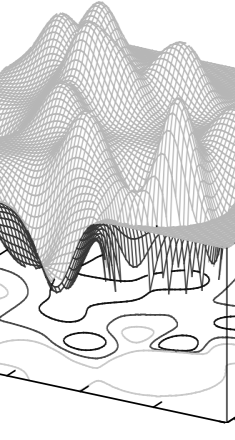
\includegraphics[height=7cm]{classPicture2-bw}
    }{\center

      \textbf{\fontsize{17}{20}\selectfont \course}

      ~

      %Lecture
      \topic\\

      \vspace{1cm}

      {\tiny~\emph{\keywords}~\\}

      \vspace{1cm}

      Marc Toussaint
      
      University of Stuttgart

      Summer 2019

      ~

    }
  }
}

\newcommand{\slide}[2]{
  \slidefont
  \incpage\begin{frame}
  \addcontentsline{toc}{section}{#1}
  \vfill
  {\headerfont #1} \vspace*{-2ex}
  \begin{itemize}\item[]~\\
    #2
  \end{itemize}
  \vfill
  \end{frame}
}

\newenvironment{slidecore}[1]{
  \slidefont\incpage
  \addcontentsline{toc}{section}{#1}
  \vfill
  {\headerfont #1} \vspace*{-2ex}
  \begin{itemize}\item[]~\\
}{
  \end{itemize}
  \vfill
}


\providecommand{\key}[1]{
  \addtocounter{mypage}{1}
% \immediate\write\keyfile{#1}
  \addtocontents{toc}{\hyperref[key:#1]{#1 (\arabic{mypage})}}
%  \phantomsection\label{key:#1}
%  \index{#1@{\hyperref[key:#1]{#1 (\arabic{mysec}:\arabic{mypage})}}|phantom}
  \addtocounter{mypage}{-1}
}

\providecommand{\course}{}

\providecommand{\subtopic}{}

\providecommand{\sublecture}[2]{
  \renewcommand{\subtopic}{#1}
  \slide{#1}{#2}
}

\providecommand{\story}[1]{
~

Motivation: {\tiny #1}\clearpage
}

\newenvironment{items}[1][9]{
\par\setlength{\unitlength}{1pt}\fontsize{#1}{#1}\linespread{1.2}\selectfont
\begin{list}{--}{\leftmargin4ex \rightmargin0ex \labelsep1ex \labelwidth2ex
\topsep0pt \parsep0ex \itemsep3pt}
}{
\end{list}
}

\providecommand{\slidesfoot}{
  \end{document}
}


  \slideshead
}

\providecommand{\exercises}{
  \newcommand{\exerciseshead}{
  \documentclass[10pt,fleqn]{article}
  \stdpackages

  \definecolor{bluecol}{rgb}{0,0,.5}
  \definecolor{greencol}{rgb}{0,.4,0}
  \definecolor{shadecolor}{gray}{0.9}
  \usepackage[
    %    pdftex%,
    %%    letterpaper,
    %    bookmarks,
    %    bookmarksnumbered,
    colorlinks,
    urlcolor=bluecol,
    citecolor=black,
    linkcolor=bluecol,
    %    pagecolor=bluecol,
    pdfborder={0 0 0},
    %pdfborderstyle={/S/U/W 1},
    %%    backref,     %link from bibliography back to sections
    %%    pagebackref, %link from bibliography back to pages
    %%    pdfstartview=FitH, %fitwidth instead of fit window
    pdfpagemode=UseNone, %UseOutlines, %bookmarks are displayed by acrobat
    pdftitle={\course},
    pdfauthor={Marc Toussaint},
    pdfkeywords={}
  ]{hyperref}
  \DeclareGraphicsExtensions{.pdf,.png,.jpg,.eps}

  \renewcommand{\r}{\varrho}
  \renewcommand{\l}{\lambda}
  \renewcommand{\L}{\Lambda}
  \renewcommand{\b}{\beta}
  \renewcommand{\d}{\delta}
  \renewcommand{\k}{\kappa}
  \renewcommand{\t}{\theta}
  \renewcommand{\O}{\Omega}
  \renewcommand{\o}{\omega}
  \renewcommand{\SS}{{\cal S}}
  \renewcommand{\=}{\!=\!}
  %\renewcommand{\boldsymbol}{}
  %\renewcommand{\Chapter}{\chapter}
  %\renewcommand{\Subsection}{\subsection}

  \renewcommand{\baselinestretch}{1.1}
  \geometry{a4paper,headsep=7mm,hdivide={15mm,*,15mm},vdivide={20mm,*,15mm}}

  \fancyhead[L]{\thetitle, \textit{Marc Toussaint}---\today}
  \fancyhead[R]{\thepage}
  \fancyhead[C]{}
  \fancyfoot{}
  \pagestyle{fancy}

  \parindent 0pt
  \parskip 0.5ex

  \newcommand{\codefont}{\helvetica{8}{1.2}{m}{n}}

  %auto-ignore
  \renewcommand{\a}{\alpha}
  \renewcommand{\b}{\beta}
  \renewcommand{\d}{\delta}
    \newcommand{\D}{\Delta}
    \newcommand{\e}{\epsilon}
    \newcommand{\g}{\gamma}
    \newcommand{\G}{\Gamma}
  \renewcommand{\l}{\lambda}
  \renewcommand{\L}{\Lambda}
    \newcommand{\m}{\mu}
    \newcommand{\n}{\nu}
    \newcommand{\N}{\nabla}
  \renewcommand{\k}{\kappa}
  \renewcommand{\o}{\omega}
  \renewcommand{\O}{\Omega}
    \newcommand{\p}{\phi}
    \newcommand{\ph}{\varphi}
  \renewcommand{\P}{\Phi}
  \renewcommand{\r}{\varrho}
    \newcommand{\s}{\sigma}
  \renewcommand{\S}{\Sigma}
  \renewcommand{\t}{\theta}
    \newcommand{\T}{\Theta}
  %\renewcommand{\v}{\vartheta}
    \newcommand{\x}{\xi}
    \newcommand{\X}{\Xi}
    \newcommand{\Y}{\Upsilon}
    \newcommand{\z}{\zeta}

  \renewcommand{\AA}{{\cal A}}
    \newcommand{\BB}{{\cal B}}
    \newcommand{\CC}{{\cal C}}
    \newcommand{\cc}{{\cal c}}
    \newcommand{\DD}{{\cal D}}
    \newcommand{\EE}{{\cal E}}
    \newcommand{\FF}{{\cal F}}
    \newcommand{\GG}{{\cal G}}
    \newcommand{\HH}{{\cal H}}
    \newcommand{\II}{{\cal I}}
    \newcommand{\KK}{{\cal K}}
    \newcommand{\LL}{{\cal L}}
    \newcommand{\MM}{{\cal M}}
    \newcommand{\NN}{{\cal N}}
    \newcommand{\oNN}{\overline\NN}
    \newcommand{\OO}{{\cal O}}
    \newcommand{\PP}{{\cal P}}
    \newcommand{\QQ}{{\cal Q}}
    \newcommand{\RR}{{\cal R}}
  \renewcommand{\SS}{{\cal S}}
    \newcommand{\TT}{{\cal T}}
    \newcommand{\uu}{{\cal u}}
    \newcommand{\UU}{{\cal U}}
    \newcommand{\VV}{{\cal V}}
    \newcommand{\XX}{{\cal X}}
    \newcommand{\xx}{\mathcal{x}}
    \newcommand{\YY}{{\cal Y}}
    \newcommand{\SOSO}{{\cal SO}}
    \newcommand{\GLGL}{{\cal GL}}

    \newcommand{\Ee}{{\rm E}}

  \newcommand{\NNN}{{\mathbb{N}}}
  \newcommand{\III}{{\mathbb{I}}}
  \newcommand{\ZZZ}{{\mathbb{Z}}}
  %\newcommand{\RRR}{{\mathrm{I\!R}}}
  \newcommand{\RRR}{{\mathbb{R}}}
  \newcommand{\SSS}{{\mathbb{S}}}
  \newcommand{\CCC}{{\mathbb{C}}}
  \newcommand{\DDD}{{\mathbb{D}}}
  \newcommand{\one}{{{\bf 1}}}
  \newcommand{\eee}{\text{e}}

  \newcommand{\NNNN}{{\overline{\cal N}}}

  \renewcommand{\[}{\Big[}
  \renewcommand{\]}{\Big]}
  \renewcommand{\(}{\Big(}
  \renewcommand{\)}{\Big)}
  \renewcommand{\|}{\,|\,}
  \renewcommand{\;}{\,;\,}
  \renewcommand{\=}{\!=\!}
    \newcommand{\<}{\left\langle}
  \renewcommand{\>}{\right\rangle}

  \newcommand{\na}[1][]{{\nabla_{\!\!#1}}}
  \newcommand{\he}[1][]{{\nabla_{\!\!#1}^2}}
  \newcommand{\Prob}{{\rm Prob}}
  \newcommand{\Dir}{{\rm Dir}}
  \newcommand{\Beta}{{\rm Beta}}
  \newcommand{\Bern}{{\rm Bern}}
  \newcommand{\Bin}{{\rm Bin}}
  \newcommand{\Mult}{{\rm Mult}}
  \newcommand{\Aut}{{\rm Aut}}
  \newcommand{\cor}{{\rm cor}}
  \newcommand{\corr}{{\rm corr}}
  \newcommand{\sd}{{\rm sd}}
  \newcommand{\tr}{{\rm tr}}
  \newcommand{\Tr}{{\rm Tr}}
  \newcommand{\rank}{{\rm rank}}
  \newcommand{\diag}{{\rm diag}}
  \newcommand{\dom}{{\rm dom}}
  \newcommand{\id}{{\rm id}}
  \newcommand{\Id}{{\rm\bf I}}
  \newcommand{\Gl}{{\rm Gl}}
  \renewcommand{\th}{\ensuremath{{}^\text{th}} }
  \newcommand{\lag}{\mathcal{L}}
  \newcommand{\inn}{\rfloor}
  \newcommand{\lie}{\pounds}
  \newcommand{\longto}{\longrightarrow}
  \newcommand{\speer}{\parbox{0.4ex}{\raisebox{0.8ex}{$\nearrow$}}}
  \renewcommand{\dag}{ {}^\dagger }
  \newcommand{\blbox}{\rule{1ex}{1ex}}
  \newcommand{\Ji}{J^\sharp}
  \newcommand{\h}{{}^\star}
  \newcommand{\w}{\wedge}
  \newcommand{\too}{\longrightarrow}
  \newcommand{\oot}{\longleftarrow}
  \newcommand{\To}{\Rightarrow}
  \newcommand{\oT}{\Leftarrow}
  \newcommand{\oTo}{\Leftrightarrow}
  \renewcommand{\iff}{~\Longleftrightarrow~}
  \newcommand{\Too}{\;\Longrightarrow\;}
  \newcommand{\oto}{\leftrightarrow}
  \newcommand{\ot}{\leftarrow}
  \newcommand{\ootoo}{\longleftrightarrow}
  \newcommand{\ow}{\stackrel{\circ}\wedge}
  \newcommand{\defeq}{\stackrel{\hspace{0.2ex}{}_\Delta}=}
%  \newcommand{\defeq}{{\overstack\Delta =}}
  \newcommand{\feed}{\nonumber \\}
  \newcommand{\comma}{~,\quad}
  \newcommand{\period}{~.\quad}
  \newcommand{\del}{\partial}
%  \newcommand{\quabla}{\Delta}
  \newcommand{\point}{$\bullet~~$}
  \newcommand{\doubletilde}{ ~ \raisebox{0.3ex}{$\widetilde {}$} \raisebox{0.6ex}{$\widetilde {}$} \!\! }
  \newcommand{\topcirc}{\parbox{0ex}{~\raisebox{2.5ex}{${}^\circ$}}}
  \newcommand{\topdot} {\parbox{0ex}{~\raisebox{2.5ex}{$\cdot$}}}
  \newcommand{\topddot} {\parbox{0ex}{~\raisebox{1.3ex}{$\ddot{~}$}}}
  \newcommand{\sym}{\topcirc}
  \newcommand{\tsum}{\textstyle\sum}
  \newcommand{\st}{\quad\text{s.t.}\quad}

  \newcommand{\half}{\ensuremath{\frac{1}{2}}}
  \newcommand{\third}{\ensuremath{\frac{1}{3}}}
  \newcommand{\fourth}{\ensuremath{\frac{1}{4}}}

  \newcommand{\ubar}{\underline}
  %\renewcommand{\vec}{\underline}
  \renewcommand{\vec}{\boldsymbol}
  %\renewcommand{\_}{\underset}
  %\renewcommand{\^}{\overset}
  %\renewcommand{\*}{{\rm\raisebox{-.6ex}{\text{*}}{}}}
  \renewcommand{\*}{\text{\footnotesize\raisebox{-.4ex}{*}{}}}

  \newcommand{\gto}{{\raisebox{.5ex}{${}_\rightarrow$}}}
  \newcommand{\gfrom}{{\raisebox{.5ex}{${}_\leftarrow$}}}
  \newcommand{\gnto}{{\raisebox{.5ex}{${}_\nrightarrow$}}}
  \newcommand{\gnfrom}{{\raisebox{.5ex}{${}_\nleftarrow$}}}

  %\newcommand{\RND}{{\SS}}
  %\newcommand{\IF}{\text{if }}
  %\newcommand{\AND}{\textsc{and }}
  %\newcommand{\OR}{\textsc{or }}
  %\newcommand{\XOR}{\textsc{xor }}
  %\newcommand{\NOT}{\textsc{not }}

  %\newcommand{\argmax}[1]{{\rm arg}\!\max_{#1}}
  %\newcommand{\argmin}[1]{{\rm arg}\!\min_{#1}}
  \DeclareMathOperator*{\argmax}{argmax}
  \DeclareMathOperator*{\argmin}{argmin}
  \DeclareMathOperator{\sign}{sign}
  \DeclareMathOperator{\acos}{acos}
  \DeclareMathOperator{\unifies}{unifies}
  \DeclareMathOperator{\Span}{span}
  \newcommand{\ortho}{\perp}
  %\newcommand{\argmax}[1]{\underset{~#1}{\text{argmax}}\;}
  %\newcommand{\argmin}[1]{\underset{~#1}{\text{argmin}}\;}
  \newcommand{\ee}[1]{\ensuremath{\cdot10^{#1}}}
  \newcommand{\sub}[1]{\ensuremath{_{\text{#1}}}}
  \newcommand{\up}[1]{\ensuremath{^{\text{#1}}}}
  \newcommand{\kld}[3][{}]{D_{#1}\big(#2\,\big|\!\big|\,#3\big)}
  %\newcommand{\kld}[2]{D\big(#1:#2\big)}
  \newcommand{\sprod}[2]{\big<#1\,,\,#2\big>}
  \newcommand{\End}{\text{End}}
  \newcommand{\txt}[1]{\quad\text{#1}\quad}
  \newcommand{\Over}[2]{\genfrac{}{}{0pt}{0}{#1}{#2}}
  %\newcommand{\mat}[1]{{\bf #1}}
  \newcommand{\arr}[2]{\hspace*{-.5ex}\begin{array}{#1}#2\end{array}\hspace*{-.5ex}}
  \newcommand{\mat}[3][.9]{
    \renewcommand{\arraystretch}{#1}{\scriptscriptstyle{\left(
      \hspace*{-1ex}\begin{array}{#2}#3\end{array}\hspace*{-1ex}
    \right)}}\renewcommand{\arraystretch}{1.2}
  }
  \newcommand{\Mat}[3][.9]{
    \renewcommand{\arraystretch}{#1}{\scriptscriptstyle{\left[
      \hspace*{-1ex}\begin{array}{#2}#3\end{array}\hspace*{-1ex}
    \right]}}\renewcommand{\arraystretch}{1.2}
  }
  \newcommand{\case}[2][ll]{\left\{\arr{#1}{#2}\right.}
  \newcommand{\seq}[1]{\textsf{\<#1\>}}
  \newcommand{\seqq}[1]{\textsf{#1}}
  \newcommand{\floor}[1]{\lfloor#1\rfloor}
  \newcommand{\Exp}[2][]{\text{E}_{#1}\{#2\}}
  \newcommand{\Var}[2][]{\text{Var}_{#1}\{#2\}}
  \newcommand{\cov}[2][]{\text{cov}_{#1}\{#2\}}

  %\newcommand{\Exp}[2]{\left\langle{#2}\right\rangle_{#1}}
  \newcommand{\ex}{\setminus}

  \providecommand{\href}[2]{{\color{blue}USE PDFLATEX!}}
  \providecommand{\url}[2]{\href{#1}{{\color{blue}#2}}}
%  \newcommand{\link}[1]{\href{{\protect #1}}{\texttt{\protect #1}}}
  \newcommand{\anchor}[2]{\begin{picture}(0,0)\put(#1){#2}\end{picture}}
  \newcommand{\pagebox}{\begin{picture}(0,0)\put(-3,-23){
    \textcolor[rgb]{.5,1,.5}{\framebox[\textwidth]{\rule[-\textheight]{0pt}{0pt}}}}
    \end{picture}}

  \newcommand{\hide}[1]{
    \begin{list}{}{\leftmargin0ex \rightmargin0ex \topsep0ex \parsep0ex}
       \helvetica{5}{1}{m}{n}
       \renewcommand{\section}{\par SECTION: }
       \renewcommand{\subsection}{\par SUBSECTION: }
       \item[$~~\blacktriangleright$]
       #1%$\blacktriangleleft~~$
       \message{^^JHIDE--Warning!^^J}
    \end{list}
  }
  %\newcommand{\hide}[1]{{\tt[hide:~}{\footnotesize\sf #1}{\tt]}\message{^^JHIDE--Warning!^^J}}
  \newcommand{\Hide}{\renewcommand{\hide}[1]{\message{^^JHIDE--Warning (hidden)!^^J}}}
  \newcommand{\HIDE}{\renewcommand{\hide}[1]{}}
  \newcommand{\fullhide}[1]{\message{^^JHIDE--Warning (hidden)!^^J}}
  \newcommand{\todo}[1]{{\tt[TODO: #1]}\message{^^JTODO--Warning: #1^^J}}
  \newcommand{\Todo}{\renewcommand{\todo}[1]{\message{^^JTODO--Warning (hidden)!^^J}}}
  %\renewcommand{\title}[1]{\renewcommand{\thetitle}{#1}}
  \newcommand{\myauthor}[1]{\author{#1}\newcommand{\theauthor}{#1}}%\@author}
  \newcommand{\mytitle}[1]{\title{#1}\newcommand{\thetitle}{#1}}%\@title}
  \newcommand{\header}{\begin{document}\mytitle\cleardefs}
  \newcommand{\contents}{{\tableofcontents}\renewcommand{\contents}{}}
  \newcommand{\footer}{\small\bibliography{marc,bibs}\end{document}}
  \newcommand{\widepaper}{\usepackage{geometry}\geometry{a4paper,hdivide={25mm,*,25mm},vdivide={25mm,*,25mm}}}
  \newcommand{\moviex}[2]{\movie[externalviewer]{#1}{#2}} %\pdflatex\usepackage{multimedia}
  \newcommand{\rbox}[1]{\fboxrule2mm\fcolorbox[rgb]{1,.85,.85}{1,.85,.85}{#1}}
  \newcommand{\mpage}[2]{{\begin{minipage}{#1\columnwidth}#2\end{minipage}}}
  \newcommand{\redbox}[2]{\fboxrule1mm\fcolorbox[rgb]{1,.7,.7}{1,.7,.7}{\begin{minipage}{#1\columnwidth}\center#2\end{minipage}}}
  \newcommand{\onecol}[2]{
    \begin{minipage}[c]{#1\columnwidth}#2\end{minipage}}
  \newcommand{\twocol}[5][0]{
    \begin{minipage}[c]{#2\columnwidth}#4\end{minipage}\hspace*{#1\columnwidth}%
    \begin{minipage}[c]{#3\columnwidth}#5\end{minipage}}
  \newcommand{\threecol}[7][0]{%
    \begin{minipage}[c]{#2\columnwidth}#5\end{minipage}\hspace*{#1\columnwidth}%
    \begin{minipage}[c]{#3\columnwidth}#6\end{minipage}\hspace*{#1\columnwidth}%
    \begin{minipage}[c]{#4\columnwidth}#7\end{minipage}}
  \newcommand{\threecoltext}[7][c]{
    \begin{minipage}[#1]{#2\textwidth}#5\end{minipage}%
    \begin{minipage}[#1]{#3\textwidth}#6\end{minipage}%
    \begin{minipage}[#1]{#4\textwidth}#7\end{minipage}}
  \newcommand{\threecoltop}[7][0]{%
   \begin{minipage}[t]{#2\columnwidth}#5\end{minipage}\hspace*{#1\columnwidth}%
   \begin{minipage}[t]{#3\columnwidth}#6\end{minipage}\hspace*{#1\columnwidth}%
   \begin{minipage}[t]{#4\columnwidth}#7\end{minipage}}
  \newcommand{\fourcol}[9][0]{%
   \begin{minipage}[c]{#2\columnwidth}#6\end{minipage}\hspace*{#1\columnwidth}%
   \begin{minipage}[c]{#3\columnwidth}#7\end{minipage}\hspace*{#1\columnwidth}%
   \begin{minipage}[c]{#4\columnwidth}#8\end{minipage}\hspace*{#1\columnwidth}%
   \begin{minipage}[c]{#5\columnwidth}#9\end{minipage}}
  \newcommand{\helvetica}[4]{\setlength{\unitlength}{1pt}\fontsize{#1}{#1}\linespread{#2}\usefont{OT1}{phv}{#3}{#4}}
  \newcommand{\helve}[1]{\helvetica{#1}{1.5}{m}{n}}
  \newcommand{\german}{\usepackage[german]{babel}\usepackage[utf8]{inputenc}}

\newcommand{\norm}[1]{|\!|#1|\!|}
\newcommand{\expr}[1]{[\hspace{-.2ex}[#1]\hspace{-.2ex}]}

\newcommand{\Jwi}{J^\sharp_W}
\newcommand{\THi}{T^\sharp_H}
\newcommand{\Jci}{J^\natural_C}
\newcommand{\hJi}{{\bar J}^\sharp}
\renewcommand{\|}{\,|\,}
\renewcommand{\=}{\!=\!}
\newcommand{\myminus}{{\hspace*{-.0pt}\text{\rm -}\hspace*{-.5pt}}}
\newcommand{\myplus}{{\hspace*{-.0pt}\text{\rm +}\hspace*{-.5pt}}}
\newcommand{\1}{{\myminus1}}
\newcommand{\2}{{\myminus2}}
\newcommand{\3}{{\myminus3}}
\newcommand{\mT}{{\text{\rm -}\hspace*{-1pt}\top}}
\newcommand{\po}{{\myplus1}}
\newcommand{\pt}{{\myplus2}}
%\renewcommand{\-}{\myminus}
%\newcommand{\+}{\myplus}
\renewcommand{\T}{{\!\top\!}}
\newcommand{\xT}{{\underline x}}
\newcommand{\uT}{{\underline u}}
\newcommand{\zT}{{\underline z}}
\newcommand{\Sum}{\textstyle\sum}
\newcommand{\Int}{\textstyle\int}
\newcommand{\Prod}{\textstyle\prod}


\newenvironment{centy}{
\vspace{15mm}
\large
\hspace*{5mm}
\begin{minipage}{8cm}\it\color{blue}
}{
\end{minipage}
}

\newcommand{\old}{{\text{old}}}
\newcommand{\new}{{\text{new}}}
\newcommand{\MAP}{{\text{MAP}}}
\newcommand{\ML}{{\text{ML}}}

\newcommand{\redArrow}{\quad\anchor{0,-1}{\includegraphics[scale=.5]{figs/redArrow}}}
\newcommand{\pub}[1]{{\color{green}\helvetica{8}{1.3}{m}{n}#1\\}}
\DeclareMathOperator{\opKL}{KL}
\newcommand{\KL}[2]{\opKL\big(#1\,\big|\!\big|\,#2\big)} %\left(#1 |\!| #2\right)}

\renewcommand{\show}[2][.8]{\centerline{\includegraphics[width=#1\columnwidth]{#2}}}
\newcommand{\showh}[2][.8]{\includegraphics[width=#1\columnwidth]{#2}}
\newcommand{\shows}[2][.8]{\centerline{\includegraphics[scale=#1]{#2}}}
\newcommand{\showhs}[2][.8]{\includegraphics[scale=#1]{#2}}
\newcommand{\mov}[2]{\movie[externalviewer]{{\color{blue}\small #1}}{movies/#2}}
\newcommand{\movex}[2]{\movie[externalviewer]{#1}{#2}} %\pdflatex\usepackage{multimedia}
%\newcommand{\movgb}[1]{\hfill\movie[externalviewer]{\small[movie]}{/home/mtoussai/movies/10-goalDirectedBehavior/#1}}
\newcommand{\movh}[3][loop]{
\movie[#1]{\showh[#2]{movies/#3.png}}{movies/#3.avi}%
\movie[externalviewer]{$\circ$}{movies/#3.avi}
}
\newcommand{\movc}[3][loop]{\centerline{\movh[#1]{#2}{#3}}}
\newcommand{\cen}[1]{\centerline{#1}}

\newcommand{\citing}[1]{
{\color{citcol}\tiny#1\par}
}

\newcommand{\cit}[3]{
\par\smallskip
{\color{greencol}\tiny #1: \emph{#2}. #3 \par}
}

\newcommand{\citurl}[4]{
\par\smallskip
{\color{greencol}\tiny #1: \protect{\href{#4}{\color{blue}{#2.}}} #3 \par}
}

\newcommand{\cito}[3]{
\par\smallskip
{\color{bluecol}\tiny #1: \emph{#2}. #3 \par}
}

\newcommand{\redoMacrosInProof}{
  \renewcommand{\d}{\delta}
%  \renewcommand{\|}{\,|\,}
  \renewcommand{\=}{\!=\!}
}

%% \makeatletter
%% \newenvironment{code}{%
%%   \begin{lrbox}{\@tempboxa}\begin{minipage}{1\columnwidth}\codefont
%% }{
%%   \end{minipage}\end{lrbox}%
%%   \colorbox[rgb]{.95,.95,.95}{\usebox{\@tempboxa}}
%% }\makeatother

\newenvironment{code}{%
\codefont
\begin{shaded}
}{
\end{shaded}
}

%\newcommand{\refeq}[1]{(\ref{#1})}

\usepackage{algorithm}
\usepackage{algpseudocode}
\algrenewcommand{\algorithmicrequire}{\textbf{Input:~~}}
\algrenewcommand{\algorithmicensure}{\textbf{Output:}}
\algrenewcommand{\algorithmiccomment}[1]{\qquad\hfill~\hspace*{-5ex}\textit{// #1}}
\algrenewcommand{\alglinenumber}[1]{\helvetica{6}{1.3}{m}{n}#1:}

\newenvironment{algo}[1][8]{
\quad\begin{minipage}{.8\columnwidth}\helvetica{#1}{1.3}{m}{n}
\medskip\hrule\medskip
\begin{algorithmic}[1]
}{
\end{algorithmic}
\medskip\hrule\medskip
\end{minipage}
}

\usepackage{etoolbox}

%%%%%%%%%%%%%%%%%%%%%%%%%%%%%%%%%%%%%%%%%%%%%%%%%%%%%%%%%%%%%%%%%%%%%%%%%%%%%%%%

\usepackage{multirow}
\usepackage{colortbl}
%\setlength{\jot}{0pt}
%\setlength{\mathindent}{1ex}
\usepackage{empheq}

%%%%%%%%%%%%%%%%%%%%%%%%%%%%%%%%%%%%%%%%%%%%%%%%%%%%%%%%%%%%%%%%%%%%%%%%%%%%%%%

\newcommand{\mypause}{\pause}
%\newcommand{\dom}{{\text{dom}}}
\newcommand{\defi}[1]{\textbf{#1}}
\newcommand{\red}[1]{\emph{\color{red}#1}}
%\newcommand{\ul}{\underline}
\newcommand{\pos}{{\textsf{pos}}}
\newcommand{\eff}{{\textsf{eff}}}
\newcommand{\rot}{{\textsf{rot}}}
\newcommand{\veC}{{\textsf{vec}}}
\newcommand{\quat}{{\textsf{quat}}}
\newcommand{\col}{{\textsf{col}}}
\newcommand{\de}[2]{\frac{\partial #1}{\partial #2}}
\newcommand{\target}{{\text{target}}}
\newcommand{\near}{{\text{near}}}
\newcommand{\qfree}{Q_{\text{free}}}
\renewcommand{\vec}{\boldsymbol}
\newcommand{\lft}{\text{left}}
\newcommand{\rgh}{\text{right}}
\DeclareMathOperator{\real}{real}
\newcommand{\prev}{{\text{prev}}}
\newcommand{\TR}[2]{T_{{#1}\shortrightarrow{#2}}}
\newcommand{\RO}[2]{R_{{#1}\shortrightarrow{#2}}}
\newcommand{\liter}{\helvetica{8}{1.1}{m}{n}\parskip 1ex}
\newcommand{\Fc}{\color{green}F}
\newcommand{\muc}{\color{blue}\mu}
\newcommand{\Astar}{A$^*$}

%for optimization course:
\newcommand{\adec}{\r_\a^-}
\newcommand{\ainc}{\r_\a^+}
\newcommand{\ldec}{\r_\l^-}
\newcommand{\linc}{\r_\l^+}
\newcommand{\minc}{\r_\m^+}
\newcommand{\mdec}{\r_\m^-}
\newcommand{\lsstop}{\r_{\text{ls}}}


\definecolor{boxcol}{rgb}{.85,.9,.92}
\newcommand{\eqbox}[1]{\centerline{\fboxrule0mm\fcolorbox{boxcol}{boxcol}{#1}}}
\newcommand{\movgb}[1]{\hfill\movie[externalviewer]{\small[movie]}{/home/mtoussai/movies/10-goalDirectedBehavior/#1}}
\newcommand{\demo}[1]{{{\color{blue}[\small #1]}}}

\graphicspath{{../pics-robotics/}{../pics-ML/}{../pics-all/}{../pics-all2/}{../pics-Optim/}}
\DeclareGraphicsExtensions{.pdf,.png,.jpg}

%\usepackage{pdfpages}
%\setbeamercolor{background canvas}{bg=}

\newcommand{\SUM}{\texttt{sum}}
\usepackage{float}

%% prevent pagebreaks before environment
\makeatletter
\newcommand{\NewParNoBreak}[1][\parskip]{\par\vspace*{-\parskip}\vspace*{#1}\nobreak\@afterheading}
\makeatother

%\newcommand{\idx}[2]{\label{IKgn}}

%%%%%%%%%%%%%%%%%%%%%%%%%%%%%%%%%%%%%%%%%%%%%%%%%%%%%%%%%%%%%%%%%%%%%%%%%%%%%%%%



%% \newwrite\tempfile
%% \immediate\openout\tempfile=z.keys.tex

%% \renewcommand{\key}[1]{
%% %%   \addtocounter{mypage}{1}
%% \makeatletter
%% \immediate\write\tempfile{\symbol{`\\}}
%% \makeatother
%%   \immediate\write\tempfile{hyperref[key:#1]{#1(\arabic{mypage})}}
%% %%  % \phantomsection\label{key:#1}
%% %%   %\index{#1@{\hyperref[key:#1]{#1 (\arabic{mysec}:\arabic{mypage})}}|phantom}
%% %%   \addtocounter{mypage}{-1}
%% }


  \DefineShortVerb{\@}

  \newcounter{solutions}
  \setcounter{solutions}{1}
  \newenvironment{solution}{
    \small
    \begin{shaded}
  }{
    \end{shaded}
  }
  
  \renewcommand{\hat}{\widehat}
  \newcommand{\bbg}{{\bar{\bar g}}}
  \graphicspath{{pics/}{../shared/pics/}}

  \renewcommand{\labelenumi}{{\alph{enumi})}}

  %%%%%%%%%%%%%%%%%%%%%%%%%%%%%%%%%%%%%%%%%%%%%%%%%%%%%%%%%%%%%%%%%%%%%%%%%%%%%%%%


  \mytitle{\course\\Exercise \exnum}
  \myauthor{Marc Toussaint\\ TAs: Janik Hager, Philipp Kratzer\\\small\addressUSTT}
  
  
  \begin{document}
  \onecolumn
  \maketitle
}

\newcommand{\exsection}[1]{\section{#1}}

\newcommand{\exerfoot}{
  \end{document}
}

\newenvironment{items}[1][9]{
  \par\setlength{\unitlength}{1pt}\fontsize{#1}{#1}\linespread{1.2}\selectfont
  \begin{list}{--}{\leftmargin4ex \rightmargin0ex \labelsep1ex \labelwidth2ex
      \topsep0pt \parsep0ex \itemsep3pt}
}{
  \end{list}
}

  \exerciseshead
}

\providecommand{\script}{
  \newcommand{\scripthead}{
  \documentclass[9pt,twoside]{article}
  \stdpackages

  \usepackage{palatino}
  \usepackage[envcountsect]{beamerarticle}
  \usepackage{makeidx}
  \makeindex

  \definecolor{bluecol}{rgb}{0,0,.5}
  \definecolor{greencol}{rgb}{0,.4,0}
  \definecolor{shadecolor}{gray}{0.9}
  \usepackage[
    %    pdftex%,
    %%    letterpaper,
    %bookmarks,
    bookmarksnumbered,
    colorlinks,
    urlcolor=bluecol,
    citecolor=black,
    linkcolor=bluecol,
    %    pagecolor=bluecol,
    pdfborder={0 0 0},
    %pdfborderstyle={/S/U/W 1},
    %%    backref,     %link from bibliography back to sections
    %%    pagebackref, %link from bibliography back to pages
    %%    pdfstartview=FitH, %fitwidth instead of fit window
    pdfpagemode=UseOutlines, %bookmarks are displayed by acrobat
    pdftitle={\course},
    pdfauthor={Marc Toussaint},
    pdfkeywords={}
  ]{hyperref}
  \DeclareGraphicsExtensions{.pdf,.png,.jpg,.eps}

  \usepackage{multimedia}
  %\setbeamercolor{background canvas}{bg=}

  \renewcommand{\r}{\varrho}
  \renewcommand{\l}{\lambda}
  \renewcommand{\L}{\Lambda}
  \renewcommand{\b}{\beta}
  \renewcommand{\d}{\delta}
  \renewcommand{\k}{\kappa}
  \renewcommand{\t}{\theta}
  \renewcommand{\O}{\Omega}
  \renewcommand{\o}{\omega}
  \renewcommand{\SS}{{\cal S}}
  \renewcommand{\=}{\!=\!}
  %\renewcommand{\boldsymbol}{}
  %\renewcommand{\Chapter}{\chapter}
  %\renewcommand{\Subsection}{\subsection}

  \renewcommand{\baselinestretch}{1.0}
  \geometry{a5paper,headsep=6mm,hdivide={10mm,*,10mm},vdivide={13mm,*,7mm}}

  \fancyhead[OL,ER]{\course, \textit{Marc Toussaint}}
  \fancyhead[OR,EL]{\thepage}
  \fancyhead[C]{}
  \fancyfoot{}
  \pagestyle{fancy}

%  \setcounter{tocdepth}{3}
  \setcounter{tocdepth}{2}

   \columnsep 6ex
  %  \renewcommand{\familydefault}{\sfdefault}
  \newcommand{\headerfont}{\large}%helvetica{12}{1}{b}{n}}
  \newcommand{\slidefont} {}%\helvetica{9}{1.3}{m}{n}}
  \newcommand{\storyfont} {}
  %  \renewcommand{\small}   {\helvetica{8}{1.2}{m}{n}}
  \renewcommand{\tiny}    {\footnotesize}%helvetica{7}{1.1}{m}{n}}
  \newcommand{\codefont}{\fontsize{6}{6}\selectfont}%helvetica{8}{1.2}{m}{n}}

  %auto-ignore
  \renewcommand{\a}{\alpha}
  \renewcommand{\b}{\beta}
  \renewcommand{\d}{\delta}
    \newcommand{\D}{\Delta}
    \newcommand{\e}{\epsilon}
    \newcommand{\g}{\gamma}
    \newcommand{\G}{\Gamma}
  \renewcommand{\l}{\lambda}
  \renewcommand{\L}{\Lambda}
    \newcommand{\m}{\mu}
    \newcommand{\n}{\nu}
    \newcommand{\N}{\nabla}
  \renewcommand{\k}{\kappa}
  \renewcommand{\o}{\omega}
  \renewcommand{\O}{\Omega}
    \newcommand{\p}{\phi}
    \newcommand{\ph}{\varphi}
  \renewcommand{\P}{\Phi}
  \renewcommand{\r}{\varrho}
    \newcommand{\s}{\sigma}
  \renewcommand{\S}{\Sigma}
  \renewcommand{\t}{\theta}
    \newcommand{\T}{\Theta}
  %\renewcommand{\v}{\vartheta}
    \newcommand{\x}{\xi}
    \newcommand{\X}{\Xi}
    \newcommand{\Y}{\Upsilon}
    \newcommand{\z}{\zeta}

  \renewcommand{\AA}{{\cal A}}
    \newcommand{\BB}{{\cal B}}
    \newcommand{\CC}{{\cal C}}
    \newcommand{\cc}{{\cal c}}
    \newcommand{\DD}{{\cal D}}
    \newcommand{\EE}{{\cal E}}
    \newcommand{\FF}{{\cal F}}
    \newcommand{\GG}{{\cal G}}
    \newcommand{\HH}{{\cal H}}
    \newcommand{\II}{{\cal I}}
    \newcommand{\KK}{{\cal K}}
    \newcommand{\LL}{{\cal L}}
    \newcommand{\MM}{{\cal M}}
    \newcommand{\NN}{{\cal N}}
    \newcommand{\oNN}{\overline\NN}
    \newcommand{\OO}{{\cal O}}
    \newcommand{\PP}{{\cal P}}
    \newcommand{\QQ}{{\cal Q}}
    \newcommand{\RR}{{\cal R}}
  \renewcommand{\SS}{{\cal S}}
    \newcommand{\TT}{{\cal T}}
    \newcommand{\uu}{{\cal u}}
    \newcommand{\UU}{{\cal U}}
    \newcommand{\VV}{{\cal V}}
    \newcommand{\XX}{{\cal X}}
    \newcommand{\xx}{\mathcal{x}}
    \newcommand{\YY}{{\cal Y}}
    \newcommand{\SOSO}{{\cal SO}}
    \newcommand{\GLGL}{{\cal GL}}

    \newcommand{\Ee}{{\rm E}}

  \newcommand{\NNN}{{\mathbb{N}}}
  \newcommand{\III}{{\mathbb{I}}}
  \newcommand{\ZZZ}{{\mathbb{Z}}}
  %\newcommand{\RRR}{{\mathrm{I\!R}}}
  \newcommand{\RRR}{{\mathbb{R}}}
  \newcommand{\SSS}{{\mathbb{S}}}
  \newcommand{\CCC}{{\mathbb{C}}}
  \newcommand{\DDD}{{\mathbb{D}}}
  \newcommand{\one}{{{\bf 1}}}
  \newcommand{\eee}{\text{e}}

  \newcommand{\NNNN}{{\overline{\cal N}}}

  \renewcommand{\[}{\Big[}
  \renewcommand{\]}{\Big]}
  \renewcommand{\(}{\Big(}
  \renewcommand{\)}{\Big)}
  \renewcommand{\|}{\,|\,}
  \renewcommand{\;}{\,;\,}
  \renewcommand{\=}{\!=\!}
    \newcommand{\<}{\left\langle}
  \renewcommand{\>}{\right\rangle}

  \newcommand{\na}[1][]{{\nabla_{\!\!#1}}}
  \newcommand{\he}[1][]{{\nabla_{\!\!#1}^2}}
  \newcommand{\Prob}{{\rm Prob}}
  \newcommand{\Dir}{{\rm Dir}}
  \newcommand{\Beta}{{\rm Beta}}
  \newcommand{\Bern}{{\rm Bern}}
  \newcommand{\Bin}{{\rm Bin}}
  \newcommand{\Mult}{{\rm Mult}}
  \newcommand{\Aut}{{\rm Aut}}
  \newcommand{\cor}{{\rm cor}}
  \newcommand{\corr}{{\rm corr}}
  \newcommand{\sd}{{\rm sd}}
  \newcommand{\tr}{{\rm tr}}
  \newcommand{\Tr}{{\rm Tr}}
  \newcommand{\rank}{{\rm rank}}
  \newcommand{\diag}{{\rm diag}}
  \newcommand{\dom}{{\rm dom}}
  \newcommand{\id}{{\rm id}}
  \newcommand{\Id}{{\rm\bf I}}
  \newcommand{\Gl}{{\rm Gl}}
  \renewcommand{\th}{\ensuremath{{}^\text{th}} }
  \newcommand{\lag}{\mathcal{L}}
  \newcommand{\inn}{\rfloor}
  \newcommand{\lie}{\pounds}
  \newcommand{\longto}{\longrightarrow}
  \newcommand{\speer}{\parbox{0.4ex}{\raisebox{0.8ex}{$\nearrow$}}}
  \renewcommand{\dag}{ {}^\dagger }
  \newcommand{\blbox}{\rule{1ex}{1ex}}
  \newcommand{\Ji}{J^\sharp}
  \newcommand{\h}{{}^\star}
  \newcommand{\w}{\wedge}
  \newcommand{\too}{\longrightarrow}
  \newcommand{\oot}{\longleftarrow}
  \newcommand{\To}{\Rightarrow}
  \newcommand{\oT}{\Leftarrow}
  \newcommand{\oTo}{\Leftrightarrow}
  \renewcommand{\iff}{~\Longleftrightarrow~}
  \newcommand{\Too}{\;\Longrightarrow\;}
  \newcommand{\oto}{\leftrightarrow}
  \newcommand{\ot}{\leftarrow}
  \newcommand{\ootoo}{\longleftrightarrow}
  \newcommand{\ow}{\stackrel{\circ}\wedge}
  \newcommand{\defeq}{\stackrel{\hspace{0.2ex}{}_\Delta}=}
%  \newcommand{\defeq}{{\overstack\Delta =}}
  \newcommand{\feed}{\nonumber \\}
  \newcommand{\comma}{~,\quad}
  \newcommand{\period}{~.\quad}
  \newcommand{\del}{\partial}
%  \newcommand{\quabla}{\Delta}
  \newcommand{\point}{$\bullet~~$}
  \newcommand{\doubletilde}{ ~ \raisebox{0.3ex}{$\widetilde {}$} \raisebox{0.6ex}{$\widetilde {}$} \!\! }
  \newcommand{\topcirc}{\parbox{0ex}{~\raisebox{2.5ex}{${}^\circ$}}}
  \newcommand{\topdot} {\parbox{0ex}{~\raisebox{2.5ex}{$\cdot$}}}
  \newcommand{\topddot} {\parbox{0ex}{~\raisebox{1.3ex}{$\ddot{~}$}}}
  \newcommand{\sym}{\topcirc}
  \newcommand{\tsum}{\textstyle\sum}
  \newcommand{\st}{\quad\text{s.t.}\quad}

  \newcommand{\half}{\ensuremath{\frac{1}{2}}}
  \newcommand{\third}{\ensuremath{\frac{1}{3}}}
  \newcommand{\fourth}{\ensuremath{\frac{1}{4}}}

  \newcommand{\ubar}{\underline}
  %\renewcommand{\vec}{\underline}
  \renewcommand{\vec}{\boldsymbol}
  %\renewcommand{\_}{\underset}
  %\renewcommand{\^}{\overset}
  %\renewcommand{\*}{{\rm\raisebox{-.6ex}{\text{*}}{}}}
  \renewcommand{\*}{\text{\footnotesize\raisebox{-.4ex}{*}{}}}

  \newcommand{\gto}{{\raisebox{.5ex}{${}_\rightarrow$}}}
  \newcommand{\gfrom}{{\raisebox{.5ex}{${}_\leftarrow$}}}
  \newcommand{\gnto}{{\raisebox{.5ex}{${}_\nrightarrow$}}}
  \newcommand{\gnfrom}{{\raisebox{.5ex}{${}_\nleftarrow$}}}

  %\newcommand{\RND}{{\SS}}
  %\newcommand{\IF}{\text{if }}
  %\newcommand{\AND}{\textsc{and }}
  %\newcommand{\OR}{\textsc{or }}
  %\newcommand{\XOR}{\textsc{xor }}
  %\newcommand{\NOT}{\textsc{not }}

  %\newcommand{\argmax}[1]{{\rm arg}\!\max_{#1}}
  %\newcommand{\argmin}[1]{{\rm arg}\!\min_{#1}}
  \DeclareMathOperator*{\argmax}{argmax}
  \DeclareMathOperator*{\argmin}{argmin}
  \DeclareMathOperator{\sign}{sign}
  \DeclareMathOperator{\acos}{acos}
  \DeclareMathOperator{\unifies}{unifies}
  \DeclareMathOperator{\Span}{span}
  \newcommand{\ortho}{\perp}
  %\newcommand{\argmax}[1]{\underset{~#1}{\text{argmax}}\;}
  %\newcommand{\argmin}[1]{\underset{~#1}{\text{argmin}}\;}
  \newcommand{\ee}[1]{\ensuremath{\cdot10^{#1}}}
  \newcommand{\sub}[1]{\ensuremath{_{\text{#1}}}}
  \newcommand{\up}[1]{\ensuremath{^{\text{#1}}}}
  \newcommand{\kld}[3][{}]{D_{#1}\big(#2\,\big|\!\big|\,#3\big)}
  %\newcommand{\kld}[2]{D\big(#1:#2\big)}
  \newcommand{\sprod}[2]{\big<#1\,,\,#2\big>}
  \newcommand{\End}{\text{End}}
  \newcommand{\txt}[1]{\quad\text{#1}\quad}
  \newcommand{\Over}[2]{\genfrac{}{}{0pt}{0}{#1}{#2}}
  %\newcommand{\mat}[1]{{\bf #1}}
  \newcommand{\arr}[2]{\hspace*{-.5ex}\begin{array}{#1}#2\end{array}\hspace*{-.5ex}}
  \newcommand{\mat}[3][.9]{
    \renewcommand{\arraystretch}{#1}{\scriptscriptstyle{\left(
      \hspace*{-1ex}\begin{array}{#2}#3\end{array}\hspace*{-1ex}
    \right)}}\renewcommand{\arraystretch}{1.2}
  }
  \newcommand{\Mat}[3][.9]{
    \renewcommand{\arraystretch}{#1}{\scriptscriptstyle{\left[
      \hspace*{-1ex}\begin{array}{#2}#3\end{array}\hspace*{-1ex}
    \right]}}\renewcommand{\arraystretch}{1.2}
  }
  \newcommand{\case}[2][ll]{\left\{\arr{#1}{#2}\right.}
  \newcommand{\seq}[1]{\textsf{\<#1\>}}
  \newcommand{\seqq}[1]{\textsf{#1}}
  \newcommand{\floor}[1]{\lfloor#1\rfloor}
  \newcommand{\Exp}[2][]{\text{E}_{#1}\{#2\}}
  \newcommand{\Var}[2][]{\text{Var}_{#1}\{#2\}}
  \newcommand{\cov}[2][]{\text{cov}_{#1}\{#2\}}

  %\newcommand{\Exp}[2]{\left\langle{#2}\right\rangle_{#1}}
  \newcommand{\ex}{\setminus}

  \providecommand{\href}[2]{{\color{blue}USE PDFLATEX!}}
  \providecommand{\url}[2]{\href{#1}{{\color{blue}#2}}}
%  \newcommand{\link}[1]{\href{{\protect #1}}{\texttt{\protect #1}}}
  \newcommand{\anchor}[2]{\begin{picture}(0,0)\put(#1){#2}\end{picture}}
  \newcommand{\pagebox}{\begin{picture}(0,0)\put(-3,-23){
    \textcolor[rgb]{.5,1,.5}{\framebox[\textwidth]{\rule[-\textheight]{0pt}{0pt}}}}
    \end{picture}}

  \newcommand{\hide}[1]{
    \begin{list}{}{\leftmargin0ex \rightmargin0ex \topsep0ex \parsep0ex}
       \helvetica{5}{1}{m}{n}
       \renewcommand{\section}{\par SECTION: }
       \renewcommand{\subsection}{\par SUBSECTION: }
       \item[$~~\blacktriangleright$]
       #1%$\blacktriangleleft~~$
       \message{^^JHIDE--Warning!^^J}
    \end{list}
  }
  %\newcommand{\hide}[1]{{\tt[hide:~}{\footnotesize\sf #1}{\tt]}\message{^^JHIDE--Warning!^^J}}
  \newcommand{\Hide}{\renewcommand{\hide}[1]{\message{^^JHIDE--Warning (hidden)!^^J}}}
  \newcommand{\HIDE}{\renewcommand{\hide}[1]{}}
  \newcommand{\fullhide}[1]{\message{^^JHIDE--Warning (hidden)!^^J}}
  \newcommand{\todo}[1]{{\tt[TODO: #1]}\message{^^JTODO--Warning: #1^^J}}
  \newcommand{\Todo}{\renewcommand{\todo}[1]{\message{^^JTODO--Warning (hidden)!^^J}}}
  %\renewcommand{\title}[1]{\renewcommand{\thetitle}{#1}}
  \newcommand{\myauthor}[1]{\author{#1}\newcommand{\theauthor}{#1}}%\@author}
  \newcommand{\mytitle}[1]{\title{#1}\newcommand{\thetitle}{#1}}%\@title}
  \newcommand{\header}{\begin{document}\mytitle\cleardefs}
  \newcommand{\contents}{{\tableofcontents}\renewcommand{\contents}{}}
  \newcommand{\footer}{\small\bibliography{marc,bibs}\end{document}}
  \newcommand{\widepaper}{\usepackage{geometry}\geometry{a4paper,hdivide={25mm,*,25mm},vdivide={25mm,*,25mm}}}
  \newcommand{\moviex}[2]{\movie[externalviewer]{#1}{#2}} %\pdflatex\usepackage{multimedia}
  \newcommand{\rbox}[1]{\fboxrule2mm\fcolorbox[rgb]{1,.85,.85}{1,.85,.85}{#1}}
  \newcommand{\mpage}[2]{{\begin{minipage}{#1\columnwidth}#2\end{minipage}}}
  \newcommand{\redbox}[2]{\fboxrule1mm\fcolorbox[rgb]{1,.7,.7}{1,.7,.7}{\begin{minipage}{#1\columnwidth}\center#2\end{minipage}}}
  \newcommand{\onecol}[2]{
    \begin{minipage}[c]{#1\columnwidth}#2\end{minipage}}
  \newcommand{\twocol}[5][0]{
    \begin{minipage}[c]{#2\columnwidth}#4\end{minipage}\hspace*{#1\columnwidth}%
    \begin{minipage}[c]{#3\columnwidth}#5\end{minipage}}
  \newcommand{\threecol}[7][0]{%
    \begin{minipage}[c]{#2\columnwidth}#5\end{minipage}\hspace*{#1\columnwidth}%
    \begin{minipage}[c]{#3\columnwidth}#6\end{minipage}\hspace*{#1\columnwidth}%
    \begin{minipage}[c]{#4\columnwidth}#7\end{minipage}}
  \newcommand{\threecoltext}[7][c]{
    \begin{minipage}[#1]{#2\textwidth}#5\end{minipage}%
    \begin{minipage}[#1]{#3\textwidth}#6\end{minipage}%
    \begin{minipage}[#1]{#4\textwidth}#7\end{minipage}}
  \newcommand{\threecoltop}[7][0]{%
   \begin{minipage}[t]{#2\columnwidth}#5\end{minipage}\hspace*{#1\columnwidth}%
   \begin{minipage}[t]{#3\columnwidth}#6\end{minipage}\hspace*{#1\columnwidth}%
   \begin{minipage}[t]{#4\columnwidth}#7\end{minipage}}
  \newcommand{\fourcol}[9][0]{%
   \begin{minipage}[c]{#2\columnwidth}#6\end{minipage}\hspace*{#1\columnwidth}%
   \begin{minipage}[c]{#3\columnwidth}#7\end{minipage}\hspace*{#1\columnwidth}%
   \begin{minipage}[c]{#4\columnwidth}#8\end{minipage}\hspace*{#1\columnwidth}%
   \begin{minipage}[c]{#5\columnwidth}#9\end{minipage}}
  \newcommand{\helvetica}[4]{\setlength{\unitlength}{1pt}\fontsize{#1}{#1}\linespread{#2}\usefont{OT1}{phv}{#3}{#4}}
  \newcommand{\helve}[1]{\helvetica{#1}{1.5}{m}{n}}
  \newcommand{\german}{\usepackage[german]{babel}\usepackage[utf8]{inputenc}}

\newcommand{\norm}[1]{|\!|#1|\!|}
\newcommand{\expr}[1]{[\hspace{-.2ex}[#1]\hspace{-.2ex}]}

\newcommand{\Jwi}{J^\sharp_W}
\newcommand{\THi}{T^\sharp_H}
\newcommand{\Jci}{J^\natural_C}
\newcommand{\hJi}{{\bar J}^\sharp}
\renewcommand{\|}{\,|\,}
\renewcommand{\=}{\!=\!}
\newcommand{\myminus}{{\hspace*{-.0pt}\text{\rm -}\hspace*{-.5pt}}}
\newcommand{\myplus}{{\hspace*{-.0pt}\text{\rm +}\hspace*{-.5pt}}}
\newcommand{\1}{{\myminus1}}
\newcommand{\2}{{\myminus2}}
\newcommand{\3}{{\myminus3}}
\newcommand{\mT}{{\text{\rm -}\hspace*{-1pt}\top}}
\newcommand{\po}{{\myplus1}}
\newcommand{\pt}{{\myplus2}}
%\renewcommand{\-}{\myminus}
%\newcommand{\+}{\myplus}
\renewcommand{\T}{{\!\top\!}}
\newcommand{\xT}{{\underline x}}
\newcommand{\uT}{{\underline u}}
\newcommand{\zT}{{\underline z}}
\newcommand{\Sum}{\textstyle\sum}
\newcommand{\Int}{\textstyle\int}
\newcommand{\Prod}{\textstyle\prod}


\newenvironment{centy}{
\vspace{15mm}
\large
\hspace*{5mm}
\begin{minipage}{8cm}\it\color{blue}
}{
\end{minipage}
}

\newcommand{\old}{{\text{old}}}
\newcommand{\new}{{\text{new}}}
\newcommand{\MAP}{{\text{MAP}}}
\newcommand{\ML}{{\text{ML}}}

\newcommand{\redArrow}{\quad\anchor{0,-1}{\includegraphics[scale=.5]{figs/redArrow}}}
\newcommand{\pub}[1]{{\color{green}\helvetica{8}{1.3}{m}{n}#1\\}}
\DeclareMathOperator{\opKL}{KL}
\newcommand{\KL}[2]{\opKL\big(#1\,\big|\!\big|\,#2\big)} %\left(#1 |\!| #2\right)}

\renewcommand{\show}[2][.8]{\centerline{\includegraphics[width=#1\columnwidth]{#2}}}
\newcommand{\showh}[2][.8]{\includegraphics[width=#1\columnwidth]{#2}}
\newcommand{\shows}[2][.8]{\centerline{\includegraphics[scale=#1]{#2}}}
\newcommand{\showhs}[2][.8]{\includegraphics[scale=#1]{#2}}
\newcommand{\mov}[2]{\movie[externalviewer]{{\color{blue}\small #1}}{movies/#2}}
\newcommand{\movex}[2]{\movie[externalviewer]{#1}{#2}} %\pdflatex\usepackage{multimedia}
%\newcommand{\movgb}[1]{\hfill\movie[externalviewer]{\small[movie]}{/home/mtoussai/movies/10-goalDirectedBehavior/#1}}
\newcommand{\movh}[3][loop]{
\movie[#1]{\showh[#2]{movies/#3.png}}{movies/#3.avi}%
\movie[externalviewer]{$\circ$}{movies/#3.avi}
}
\newcommand{\movc}[3][loop]{\centerline{\movh[#1]{#2}{#3}}}
\newcommand{\cen}[1]{\centerline{#1}}

\newcommand{\citing}[1]{
{\color{citcol}\tiny#1\par}
}

\newcommand{\cit}[3]{
\par\smallskip
{\color{greencol}\tiny #1: \emph{#2}. #3 \par}
}

\newcommand{\citurl}[4]{
\par\smallskip
{\color{greencol}\tiny #1: \protect{\href{#4}{\color{blue}{#2.}}} #3 \par}
}

\newcommand{\cito}[3]{
\par\smallskip
{\color{bluecol}\tiny #1: \emph{#2}. #3 \par}
}

\newcommand{\redoMacrosInProof}{
  \renewcommand{\d}{\delta}
%  \renewcommand{\|}{\,|\,}
  \renewcommand{\=}{\!=\!}
}

%% \makeatletter
%% \newenvironment{code}{%
%%   \begin{lrbox}{\@tempboxa}\begin{minipage}{1\columnwidth}\codefont
%% }{
%%   \end{minipage}\end{lrbox}%
%%   \colorbox[rgb]{.95,.95,.95}{\usebox{\@tempboxa}}
%% }\makeatother

\newenvironment{code}{%
\codefont
\begin{shaded}
}{
\end{shaded}
}

%\newcommand{\refeq}[1]{(\ref{#1})}

\usepackage{algorithm}
\usepackage{algpseudocode}
\algrenewcommand{\algorithmicrequire}{\textbf{Input:~~}}
\algrenewcommand{\algorithmicensure}{\textbf{Output:}}
\algrenewcommand{\algorithmiccomment}[1]{\qquad\hfill~\hspace*{-5ex}\textit{// #1}}
\algrenewcommand{\alglinenumber}[1]{\helvetica{6}{1.3}{m}{n}#1:}

\newenvironment{algo}[1][8]{
\quad\begin{minipage}{.8\columnwidth}\helvetica{#1}{1.3}{m}{n}
\medskip\hrule\medskip
\begin{algorithmic}[1]
}{
\end{algorithmic}
\medskip\hrule\medskip
\end{minipage}
}

\usepackage{etoolbox}

%%%%%%%%%%%%%%%%%%%%%%%%%%%%%%%%%%%%%%%%%%%%%%%%%%%%%%%%%%%%%%%%%%%%%%%%%%%%%%%%

\usepackage{multirow}
\usepackage{colortbl}
%\setlength{\jot}{0pt}
%\setlength{\mathindent}{1ex}
\usepackage{empheq}

%%%%%%%%%%%%%%%%%%%%%%%%%%%%%%%%%%%%%%%%%%%%%%%%%%%%%%%%%%%%%%%%%%%%%%%%%%%%%%%

\newcommand{\mypause}{\pause}
%\newcommand{\dom}{{\text{dom}}}
\newcommand{\defi}[1]{\textbf{#1}}
\newcommand{\red}[1]{\emph{\color{red}#1}}
%\newcommand{\ul}{\underline}
\newcommand{\pos}{{\textsf{pos}}}
\newcommand{\eff}{{\textsf{eff}}}
\newcommand{\rot}{{\textsf{rot}}}
\newcommand{\veC}{{\textsf{vec}}}
\newcommand{\quat}{{\textsf{quat}}}
\newcommand{\col}{{\textsf{col}}}
\newcommand{\de}[2]{\frac{\partial #1}{\partial #2}}
\newcommand{\target}{{\text{target}}}
\newcommand{\near}{{\text{near}}}
\newcommand{\qfree}{Q_{\text{free}}}
\renewcommand{\vec}{\boldsymbol}
\newcommand{\lft}{\text{left}}
\newcommand{\rgh}{\text{right}}
\DeclareMathOperator{\real}{real}
\newcommand{\prev}{{\text{prev}}}
\newcommand{\TR}[2]{T_{{#1}\shortrightarrow{#2}}}
\newcommand{\RO}[2]{R_{{#1}\shortrightarrow{#2}}}
\newcommand{\liter}{\helvetica{8}{1.1}{m}{n}\parskip 1ex}
\newcommand{\Fc}{\color{green}F}
\newcommand{\muc}{\color{blue}\mu}
\newcommand{\Astar}{A$^*$}

%for optimization course:
\newcommand{\adec}{\r_\a^-}
\newcommand{\ainc}{\r_\a^+}
\newcommand{\ldec}{\r_\l^-}
\newcommand{\linc}{\r_\l^+}
\newcommand{\minc}{\r_\m^+}
\newcommand{\mdec}{\r_\m^-}
\newcommand{\lsstop}{\r_{\text{ls}}}


\definecolor{boxcol}{rgb}{.85,.9,.92}
\newcommand{\eqbox}[1]{\centerline{\fboxrule0mm\fcolorbox{boxcol}{boxcol}{#1}}}
\newcommand{\movgb}[1]{\hfill\movie[externalviewer]{\small[movie]}{/home/mtoussai/movies/10-goalDirectedBehavior/#1}}
\newcommand{\demo}[1]{{{\color{blue}[\small #1]}}}

\graphicspath{{../pics-robotics/}{../pics-ML/}{../pics-all/}{../pics-all2/}{../pics-Optim/}}
\DeclareGraphicsExtensions{.pdf,.png,.jpg}

%\usepackage{pdfpages}
%\setbeamercolor{background canvas}{bg=}

\newcommand{\SUM}{\texttt{sum}}
\usepackage{float}

%% prevent pagebreaks before environment
\makeatletter
\newcommand{\NewParNoBreak}[1][\parskip]{\par\vspace*{-\parskip}\vspace*{#1}\nobreak\@afterheading}
\makeatother

%\newcommand{\idx}[2]{\label{IKgn}}

%%%%%%%%%%%%%%%%%%%%%%%%%%%%%%%%%%%%%%%%%%%%%%%%%%%%%%%%%%%%%%%%%%%%%%%%%%%%%%%%



%% \newwrite\tempfile
%% \immediate\openout\tempfile=z.keys.tex

%% \renewcommand{\key}[1]{
%% %%   \addtocounter{mypage}{1}
%% \makeatletter
%% \immediate\write\tempfile{\symbol{`\\}}
%% \makeatother
%%   \immediate\write\tempfile{hyperref[key:#1]{#1(\arabic{mypage})}}
%% %%  % \phantomsection\label{key:#1}
%% %%   %\index{#1@{\hyperref[key:#1]{#1 (\arabic{mysec}:\arabic{mypage})}}|phantom}
%% %%   \addtocounter{mypage}{-1}
%% }


  \DefineShortVerb{\@}

  \newcounter{solutions}
  \setcounter{solutions}{1}
  \renewenvironment{solution}{
    \small
    \begin{shaded}
  }{
    \end{shaded}
  }

  \graphicspath{{pics/}{../shared/pics/}}

%%%%%%%%%%%%%%%%%%%%%%%%%%%%%%%%%%%%%%%%%%%%%%%%%%%%%%%%%%%%%%%%%%%%%%%%%%%%%%%%

  \mytitle{\course\\Lecture Script}
  \myauthor{Marc Toussaint}

  \begin{document}

  %% \vspace*{2cm}

  \maketitle
  %\anchor{100,10}{\includegraphics[width=4cm]{optim}}

%  \vspace*{1cm}

  \emph{This is a direct concatenation and reformatting of all lecture
    slides and exercises from the \emph{Machine Learning} course (summer
    term 2019, U Stuttgart), including indexing to help
    prepare for exams.}

  \emph{Double-starred** sections and slides are not relevant for the exam.}

  {\tableofcontents}
}

%%%%%%%%%%%%%%%%%%%%%%%%%%%%%%%%%%%%%%%%%%%%%%%%%%%%%%%%%%%%%%%%%%%%%%%%%%%%%%%%

%% \renewcommand{\keywords}{}
%% \newcommand{\topic}{}
%% \renewcommand{\mypause}{}

  \newcounter{mypage}
  \setcounter{mypage}{0}
  \newcounter{mysec}
  \setcounter{mysec}{0}
  \newcommand{\incpage}{\addtocounter{mypage}{1}}
  \newcommand{\incsec} {\addtocounter{mysec}{1}}

\newcommand{\beginTocMinipage}{
  \addtocontents{toc}{\smallskip\noindent\hspace*{.036\columnwidth}}
  \addtocontents{toc}{\protect\begin{minipage}{.914\columnwidth}\small}
}
\newcommand{\closeTocMinipage}{
  \addtocontents{toc}{\protect\end{minipage}}
  \addtocontents{toc}{}
  \addtocontents{toc}{\medskip}
}

\renewcommand{\slides}[1][]{
  \clearpage
  \incsec
  \section{\topic}
  {\small #1}
  \beginTocMinipage
  \setcounter{mypage}{0}
  \smallskip\nopagebreak\hrule\medskip
}

\newcommand{\slidesfoot}{
  \closeTocMinipage
  \bigskip
}

\newcommand{\sublecture}[2]{
  \pagebreak[3]
  \incpage
  \closeTocMinipage
  \subsection{#1}
  {\storyfont #2}
  \beginTocMinipage
  {\hfill\tiny \textsf{\arabic{mysec}:\arabic{mypage}}}\nopagebreak%
  \smallskip\nopagebreak\hrule
}

\newcommand{\key}[1]{
  \pagebreak[2]
  \addtocounter{mypage}{1}
  \addtocontents{toc}{\hyperref[key:#1]{#1 (\arabic{mysec}:\arabic{mypage})}}
  \phantomsection\label{key:#1}
  \index{#1@{\hyperref[key:#1]{#1 (\arabic{mysec}:\arabic{mypage})}}|phantom}
  \addtocounter{mypage}{-1}
}

\newenvironment{slidecore}[1]{
  \incpage
  \subsubsection*{#1}%{\headerfont\noindent\textbf{#1}\\}%
  \vspace{-6ex}%
  \begin{list}{$\bullet$}{\leftmargin4ex \rightmargin0ex \labelsep1ex
    \labelwidth2ex \partopsep0ex \topsep0ex \parsep.5ex \parskip0ex \itemsep0pt}\item[]~\\\nopagebreak%
}{
  \end{list}\nopagebreak%
  {\hfill\tiny \textsf{\arabic{mysec}:\arabic{mypage}}}\nopagebreak%
  \smallskip\nopagebreak\hrule
}

\newcommand{\slide}[2]{
  \begin{slidecore}{#1}
    #2
  \end{slidecore}
}

\newcommand{\exsection}[1]{
  \subsubsection{#1}
}

\renewcommand{\exercises}{
  \subsection{Exercise \exnum}
}

\newcommand{\exerfoot}{
  \bigskip
}

\newcommand{\story}[1]{
  \subsection*{Motivation \& Outline}
  \addtocontents{toc}{\hyperref[mot\arabic{mysec}]{Motivation \& Outline}}
  \phantomsection\label{mot\arabic{mysec}}
  {\storyfont\sf #1}
  \medskip\nopagebreak\hrule
}

\newcounter{savedsection}
\newcommand{\subappendix}{\setcounter{savedsection}{\arabic{section}}\appendix}
\newcommand{\noappendix}{
  \setcounter{section}{\arabic{savedsection}}% restore section number
  \setcounter{subsection}{0}% reset section counter
%  \gdef\@chapapp{\sectionname}% reset section name
  \renewcommand{\thesection}{\arabic{section}}% make section numbers arabic
}

\newenvironment{items}[1][9]{
\par\setlength{\unitlength}{1pt}\fontsize{#1}{#1}\linespread{1.2}\selectfont
\begin{list}{--}{\leftmargin4ex \rightmargin0ex \labelsep1ex \labelwidth2ex
\topsep0pt \parsep0ex \itemsep3pt}
}{
\end{list}
}

  \scripthead
}

\providecommand{\course}{NO COURSE}
\providecommand{\topic}{NO TOPIC}
\providecommand{\keywords}{NO KEYWORDS}
\providecommand{\exnum}{NO NUMBER}


\providecommand{\stdpackages}{
  \usepackage{amsmath}
  \usepackage{amssymb}
  \usepackage{amsfonts}
  \allowdisplaybreaks
  \usepackage{amsthm}
  \usepackage{eucal}
  \usepackage{graphicx}
  \usepackage{color}
  \usepackage{geometry}
  \usepackage{framed}
%  \usecolor{xcolor}
  \definecolor{shadecolor}{gray}{0.9}
  \setlength{\FrameSep}{3pt}
  \usepackage{fancyvrb}
  \fvset{numbers=left,xleftmargin=5ex}

  \usepackage{multicol} 
  \usepackage{fancyhdr}
}

\providecommand{\addressUSTT}{
  Machine~Learning~\&~Robotics~lab, U~Stuttgart\\\small
  Universit{\"a}tsstra{\ss}e 38, 70569~Stuttgart, Germany
}


\renewcommand{\course}{Machine Learning}
\renewcommand{\coursepicture}{course_ml}
\renewcommand{\coursedate}{Summer 2019}
\renewcommand{\topic}{Graphical Models}
\renewcommand{\keywords}{Bayesian Networks, conditional
independence, Sampling methods (Rejection, Importance,
Gibbs), Variable Elimination, Factor Graphs, Message passing, Loopy
Belief Propagation, Junction Tree Algorithm}

\slides

%%%%%%%%%%%%%%%%%%%%%%%%%%%%%%%%%%%%%%%%%%%%%%%%%%%%%%%%%%%%%%%%%%%%%%%%%%%%%%%%

\slide{Outline}{

\item A.~ Introduction

{\tiny
-- Motivation and definition of Bayes Nets

-- Conditional independence in Bayes Nets

-- Examples

}

\item B.~ Inference in Graphical Models

{\tiny
-- Sampling methods (Rejection, Importance,
Gibbs)

-- Variable Elimination \& Factor Graphs

-- Message passing, Loopy Belief Propagation

}

\item C.~ Learning in Graphical Models

{\tiny
-- Maximum likelihood learning

-- Expectation Maximization, Gaussian Mixture Models, Hidden Markov
Models, Free Energy formulation

-- Discriminative Learning

}

}

%%%%%%%%%%%%%%%%%%%%%%%%%%%%%%%%%%%%%%%%%%%%%%%%%%%%%%%%%%%%%%%%%%%%%%%%%%%%%%%%

\slide{Graphical Models}{

\item The core difficulty in modelling is specifying

\cen{\emph{What are the relevant variables?}}

\cen{\emph{How do they depend on each other?}}

\cen{(Or how \emph{could} they depend on each other $\to$ learning)}

~\mypause

\item \textbf{Graphical models} are a simple, graphical notation for

~~ 1) which random variables exist

~~ 2) which random variables are ``directly coupled''

Thereby they \emph{describe a joint probability distribution}
$P(X_1,..,X_n)$ over
$n$ random variables.

~\mypause

\item 2 basic variants:
\begin{items}
\item Bayesian Networks ~~ (aka.\ directed model, belief network)

\item Factor Graphs ~~ (aka.\ undirected model, Markov Random Field)
\end{items}

}

%%%%%%%%%%%%%%%%%%%%%%%%%%%%%%%%%%%%%%%%%%%%%%%%%%%%%%%%%%%%%%%%%%%%%%%%%%%%%%%%

\key{Bayesian Network}
\slide{Bayesian Networks}{

\item A \textbf{Bayesian Network} is a
\begin{items}
\item directed acyclic graph (DAG)

\item where each node represents a random variable $X_i$

\item for each node we have a conditional probability distribution

   \cen{$P(X_i \| \text{Parents}(X_i))$}
\end{items}

~

\item In the simplest case (discrete RVs), the conditional 
   distribution is represented as a conditional probability table
   (\textbf{CPT})

}

%%%%%%%%%%%%%%%%%%%%%%%%%%%%%%%%%%%%%%%%%%%%%%%%%%%%%%%%%%%%%%%%%%%%%%%%%%%%%%%%

\slide{Example}{

\cen{drinking red wine $\to$ longevity?}

}

%%%%%%%%%%%%%%%%%%%%%%%%%%%%%%%%%%%%%%%%%%%%%%%%%%%%%%%%%%%%%%%%%%%%%%%%%%%%%%%%

\slide{Bayesian Networks}{

\item DAG $\to$ we can sort the RVs; edges only go from lower to
higher index

\item  \textbf{The joint distribution can be factored as}
\begin{align*}
P(X_{1:n})
 &= \prod_{i=1}^n P(X_i \| \text{Parents}(X_i))
\end{align*}
%(notation: $X_{\pi(i)} = (X_a,..,X_b)$ if $\pi(i)=(a,..,b)$ )

\item Missing links imply conditional independence

\item Ancestral simulation to sample from joint distribution

}

%%%%%%%%%%%%%%%%%%%%%%%%%%%%%%%%%%%%%%%%%%%%%%%%%%%%%%%%%%%%%%%%%%%%%%%%%%%%%%%%

\slide{Example}{

\hfill{\tiny (Heckermann 1995)}
\show[.6]{vl2-car}

$
\iff ~ P(S,T,G,F,B) = P(B)~ P(F)~ P(G|F,B)~ P(T|B)~ P(S|T,F)
$

~

\item Table sizes: ~ LHS = $2^5-1=31$ ~ RHS = $1 + 1 + 4 + 2 + 4=12$


}

%%%%%%%%%%%%%%%%%%%%%%%%%%%%%%%%%%%%%%%%%%%%%%%%%%%%%%%%%%%%%%%%%%%%%%%%%%%%%%%%

\slide{Constructing a Bayes Net}{

\item[1.] Choose a relevant set of variables $X_i$ that describe the
domain

\item[2.] Choose an ordering for the variables

\item[3.] While there are variables left

 (a) Pick a variable $X_i$ and add it to the network

 (b) Set $\text{Parents}(X_i)$ to some minimal set of nodes already in
 the net

 (c) Define the CPT for $X_i$

}

%%%%%%%%%%%%%%%%%%%%%%%%%%%%%%%%%%%%%%%%%%%%%%%%%%%%%%%%%%%%%%%%%%%%%%%%%%%%%%%%

\slide{}{

\item This procedure is guaranteed to produce a DAG

\item Different orderings may lead to \textbf{different Bayes
nets representing the same joint distribution}:

\item To ensure maximum sparsity choose a wise order (``root
causes''first). Counter example: construct DAG for the car example
using the ordering S, T, G, F, B

\item ``Wrong'' ordering will give same
joint distribution, but will require the specification of more numbers
than otherwise necessary

}

%%%%%%%%%%%%%%%%%%%%%%%%%%%%%%%%%%%%%%%%%%%%%%%%%%%%%%%%%%%%%%%%%%%%%%%%%%%%%%%%

\key{Conditional independence in a Bayes Net}
\slide{Bayes Nets \& conditional independence}{

\item Independence: ~ $Indep(X,Y) \iff P(X,Y) = P(X)~ P(Y)$

\item Conditional independence: ~

\cen{$Indep(X,Y|Z) \iff P(X,Y | Z) = P(X|Z)~ P(Y|Z)$}

%(This implies $P(X,Y,Z) = P(X,Y | Z)~ P(Z) = P(X|Z)~ P(Y|Z)~ P(Z)$.)

~

~\mypause

\threecol{.33}{.33}{.33}{\center
\show[.7]{vl2-indep1}

(head-to-head)

~

$Indep(X,Y)$

$\neg Indep(X,Y|Z)$
}{\center
\show[.7]{vl2-indep2}

(tail-to-tail)

~

$\neg Indep(X,Y)$

$Indep(X,Y|Z)$
}{\center
\show[.7]{vl2-indep3}

(head-to-tail)

~

$\neg Indep(X,Y)$

$Indep(X,Y|Z)$
}

}

%%%%%%%%%%%%%%%%%%%%%%%%%%%%%%%%%%%%%%%%%%%%%%%%%%%%%%%%%%%%%%%%%%%%%%%%%%%%%%%%

\slide{}{


\item Head-to-head: $Indep(X, Y)$
 
$P(X, Y, Z) = P(X)~ P(Y)~ P(Z|X, Y)$

$P(X, Y) = P(X)~ P(Y)~ \sum_Z P(Z|X, Y) = P(X)~ P(Y)$

~

\item Tail-to-tail: $Indep(X, Y|Z)$

$P(X, Y, Z) = P(Z)~ P(X|Z)~ P(Y|Z)$

$P(X, Y|Z) = P(X, Y, Z) = P(Z) = P(X|Z)~ P(Y|Z)$

~

\item Head-to-tail: $Indep(X, Y|Z)$

$P(X, Y, Z) = P(X)~ P(Z|X)~ P(Y|Z)$

$P(X, Y|Z) = \frac{P(X, Y, Z)}{P(Z)} = \frac{P(X, Z)~ P(Y|Z)}{P(Z)} = P(X|Z)~
P(Y|Z)$
}

%%%%%%%%%%%%%%%%%%%%%%%%%%%%%%%%%%%%%%%%%%%%%%%%%%%%%%%%%%%%%%%%%%%%%%%%%%%%%%%%

\slide{}{

General rules for determining conditional independence in a Bayes net:

~

\item Given three groups of random variables $X,Y,Z$

~

\cen{$Indep(X,Y|Z) \iff$ every path from $X$ to $Y$ is ``blocked by $Z$''}

~

\item A path is ``blocked by $Z$'' $\iff$ on this path...
\begin{items}
\item $\exists$ a node in $Z$ that is head-to-tail w.r.t.\ the path, or

\item $\exists$ a node in $Z$ that is tail-to-tail w.r.t.\ the path, or

\item $\exists$ another node $A$ which is head-to-head w.r.t.\ the
   path\\ ~~ and neither $A$ nor any of its descendants are in $Z$
\end{items}

}

%%%%%%%%%%%%%%%%%%%%%%%%%%%%%%%%%%%%%%%%%%%%%%%%%%%%%%%%%%%%%%%%%%%%%%%%%%%%%%%%

\slide{Example}{

\hfill{\tiny (Heckermann 1995)}
\show[.6]{vl2-car}

~

\cen{ $Indep(T,F)$? ~~ $Indep(B,F|S)$? ~~ $Indep(B,S|T)$? }

}

%%%%%%%%%%%%%%%%%%%%%%%%%%%%%%%%%%%%%%%%%%%%%%%%%%%%%%%%%%%%%%%%%%%%%%%%%%%%%%%%

%% \slide{Causality?}{

%% \item Bayes nets are also called causal networks (Pearl, 1988)

%% \item We know that any joint distribution $P(X,Y)$ can be factorized
%% as
%% \twocol{.4}{.4}{$P(X,Y) = P(X|Y)~ P(Y)$}{}

%% \twocol{.4}{.4}{$P(X,Y) = P(Y|X)~ P(X)$}{}

%% Both Bayes nets are ``correct''

%% }

%%%%%%%%%%%%%%%%%%%%%%%%%%%%%%%%%%%%%%%%%%%%%%%%%%%%%%%%%%%%%%%%%%%%%%%%%%%%%%%%

\slide{What can we do with Bayes nets?}{

\item \textbf{Inference:} Given some pieces of information (prior,
  observed variabes) what is the implication (the implied information,
  the posterior) on a non-observed variable

~

\item \textbf{Learning:}
\begin{items}
\item Fully Bayesian Learning: Inference over parameters (e.g., $\b$)

\item Maximum likelihood training: Optimizing parameters
\end{items}

~

\item \textbf{Structure Learning} (Learning/Inferring the graph structure itself):
Decide which model (which graph structure) fits the data best; thereby
uncovering conditional independencies in the data.

}

%%%%%%%%%%%%%%%%%%%%%%%%%%%%%%%%%%%%%%%%%%%%%%%%%%%%%%%%%%%%%%%%%%%%%%%%%%%%%%%%

\key{Inference: general meaning}
\slide{Inference}{

\item Inference: Given some pieces of information (prior,
  observed variabes) what is the implication (the implied
  information, the posterior) on a non-observed variable

~

\item In a Bayes Nets: Assume there is three groups of RVs:
\begin{items}
\item $Z$ are observed random variables

\item $X$ and $Y$ are hidden random variables

\item We want to do inference about $X$, not $Y$
\end{items}

~

Given some observed variables $Z$, compute
the\\ \textbf{posterior marginal} $P(X \| Z)$ for some hidden
variable $X$.

~

\begin{align*}
P(X \| Z)
 &= \frac{P(X, Z)}{P(Z)}
  = \frac{1}{P(Z)}~ \sum_Y P(X,Y,Z)
\end{align*}
where $Y$ are all hidden random variables except for $X$

~

\item Inference requires summing over \emph{(eliminating)} hidden variables.

}

%%%%%%%%%%%%%%%%%%%%%%%%%%%%%%%%%%%%%%%%%%%%%%%%%%%%%%%%%%%%%%%%%%%%%%%%%%%%%%%%

\slide{Example: Holmes \& Watson}{

\item Mr. Holmes lives in Los Angeles. One morning when Holmes leaves
his house, he realizes that his grass is wet. Is it due to rain, or
has he forgotten to turn off his sprinkler?
\begin{items}
\item Calculate $P(R|H)$, $P(S|H)$ and compare these values to the prior probabilities.

\item Calculate $P(R, S|H)$.

   Note: $R$ and $S$ are marginally independent, but conditionally dependent
\end{items}

~

\item Holmes checks Watson's grass, and finds it is also wet.
\begin{items}
\item Calculate $P(R|H,W)$, $P(S|H,W)$

\item This effect is called explaining away
\end{items}

~

{\small JavaBayes: run it from the html page\\
\url{http://www.cs.cmu.edu/~javabayes/Home/applet.html} }

}

%%%%%%%%%%%%%%%%%%%%%%%%%%%%%%%%%%%%%%%%%%%%%%%%%%%%%%%%%%%%%%%%%%%%%%%%%%%%%%%%

\slide{Example: Holmes \& Watson}{

\show[0.5]{vl2-rain}
\cen{$P(H,W,S,R) = P(H|S,R)~ P(W|R)~ P(S)~ P(R)$}

\tiny
\begin{align*}
P(R|H)
 &= \sum_{W,S} \frac{P(R,W,S,H)}{P(H)}
  = \frac{1}{P(H)} \sum_{W,S} P(H|S,R)~ P(W|R)~ P(S)~ P(R) \\
 &= \frac{1}{P(H)} \sum_S P(H|S,R)~ P(S)~ P(R) \\
\hspace*{-10mm}
P(R\=1 \| H\=1)
 &= \frac{1}{P(H\=1)} (1.0 \cdot 0.2 \cdot 0.1 + 1.0 \cdot 0.2 \cdot
 0.9)
  = \frac{1}{P(H\=1)} 0.2\\
\hspace*{-10mm}
P(R\=0 \| H\=1)
 &= \frac{1}{P(H\=1)} (0.9 \cdot 0.8 \cdot 0.1 + 0.0 \cdot 0.8 \cdot
 0.9)
  = \frac{1}{P(H\=1)} 0.072
\end{align*}
}

%%%%%%%%%%%%%%%%%%%%%%%%%%%%%%%%%%%%%%%%%%%%%%%%%%%%%%%%%%%%%%%%%%%%%%%%%%%%%%%%

\slide{}{

\item These types of calculations can be automated

$\to$ Variable Elimination Algorithm

}

%%%%%%%%%%%%%%%%%%%%%%%%%%%%%%%%%%%%%%%%%%%%%%%%%%%%%%%%%%%%%%%%%%%%%%%%%%%%%%%%

\slide{Example: Bavarian dialect}{

~

\show[.05]{bavarian}

\item Two binary random variables(RVs): $B$ (bavarian) and $D$ (dialect)

\item Given:

$P(D,B) = P(D \| B)~ P(B)$

$P(D\=1 \| B\=1) = 0.4$, $P(D\=1 \| B\=0) = 0.01$, $P(B\=1) = 0.15$

~

\item \textbf{Notation:} Grey shading usually indicates ``observed''

}

%%%%%%%%%%%%%%%%%%%%%%%%%%%%%%%%%%%%%%%%%%%%%%%%%%%%%%%%%%%%%%%%%%%%%%%%%%%%%%%%

\slide{Example: Coin flipping}{

~

\show[.35]{coinFlipping}

\item  One binary RV $H$ (hypothesis), 5 RVs for the coin tosses $d_1,..,d_5$

\item Given:

$P(D,H) = \prod_i P(d_i \| H)~ P(H)$

$P(H\=1)=\frac{999}{1000}$, 
$P(d_i\=\texttt{H} \| H\=1) = \half$, $P(d_i\=\texttt{H} \| H\=2) = 1$

}

%%%%%%%%%%%%%%%%%%%%%%%%%%%%%%%%%%%%%%%%%%%%%%%%%%%%%%%%%%%%%%%%%%%%%%%%%%%%%%%%

\slide{Example: Ridge regression}{

~

\show[.2]{regression}

\item One multi-variate RV $\b$, $2n$ RVs $x_{1:n}$, $y_{1:n}$ (observed
   data)

\item Given:

$P(D ,\b) = \prod_i \[P(y_i \| x_i,\b)~ P(x_i)\]~ P(\b)$

 $P(\b) =  \NN(\b \| 0,\frac{\s^2}{\lambda})$, $P(y_i \| x_i,\b) = \NN(y_i \| x_i^\T \b, \s^2)$

~

\item \textbf{Plate notation:} Plates (boxes with index ranges) mean
``copy $n$-times''

}

%% ~

%% Gaussian Mixture Model:

%% \item Discrete latent RVs $c_{1:n}$ indicating mixture component,
%% cont.\ RVs $x_{1:n}$ (observed data)

%% \item Model: ~ $P(x_i \| \m_{1:K},\S_{1:K}) = \sum_{k=1}^K \NN(x_i \| \m_k,\S_k)~ P(c_i\=k)$
%% \anchor{10,-40}{\showh[.16]{gaussianMixture}}

%% }

%% }



%% \slide{Number of parameters}{

%% \item Representing $P(H,W,S,R)$ as big array of probabilities

%% $\to$ ~ $2^4-1 = 15$ parameters

%% ~

%% \item Representing $P(H|S,R)~ P(W|R)~ P(S)~ P(R)$ as 4 separate
%% CPTs

%% $\to$ ~ $2^2 + 2 + 1 + 1 = 8$ parameters

%% ~\mypause

%% \emph{Conditional independences reduces the number of
%% parameters $\to$ this is reflected directly also in the Bayes Net.}

%% }


%%%%%%%%%%%%%%%%%%%%%%%%%%%%%%%%%%%%%%%%%%%%%%%%%%%%%%%%%%%%%%%%%%%%%%%%%%%%%%%%

\sublecture{Inference in Graphical Models}{
}

%%%%%%%%%%%%%%%%%%%%%%%%%%%%%%%%%%%%%%%%%%%%%%%%%%%%%%%%%%%%%%%%%%%%%%%%%%%%%%%%

\key{Inference in graphical models: overview}
\slide{Common inference methods in graphical models}{

\item \textbf{Sampling:}
\begin{items}
\item Rejection samping, importance sampling, Gibbs sampling

\item More generally, Markov-Chain Monte Carlo (MCMC) methods
\end{items}

~

\item \textbf{Message passing:}
\begin{items}
\item Exact inference on trees (includes the Junction Tree Algorithm)

\item Belief propagation
\end{items}

~

\item \textbf{Other approximations/variational methods}
\begin{items}
\item Expectation propagation

\item Specialized variational methods depending on the model
\end{items}

~

\item \textbf{Reductions:}
\begin{items}
\item Mathematical Programming (e.g.\ LP relaxations of MAP)

\item Compilation into Arithmetic Circuits (Darwiche at al.)
\end{items}

}

%%%%%%%%%%%%%%%%%%%%%%%%%%%%%%%%%%%%%%%%%%%%%%%%%%%%%%%%%%%%%%%%%%%%%%%%%%%%%%%%

\slide{Probabilistic Inference \& Optimization}{

~

\show[.5]{inferenceAndOptimization}

~

\item Note the relation of the Boltzmann distribution $p(x) \propto
e^{-f(x)/T}$ with the cost function (energy) $f(x)$ and temperature $T$.

}

%%%%%%%%%%%%%%%%%%%%%%%%%%%%%%%%%%%%%%%%%%%%%%%%%%%%%%%%%%%%%%%%%%%%%%%%%%%%%%%%

\slide{Sampling}{

\item Read Andrieu
et al: \emph{An Introduction to MCMC for Machine Learning} (Machine
Learning, 2003)

~

\item Here I'll discuss only thee basic methods:
\begin{items}
\item Rejection sampling

\item Importance sampling

\item Gibbs sampling
\end{items}

}

%%%%%%%%%%%%%%%%%%%%%%%%%%%%%%%%%%%%%%%%%%%%%%%%%%%%%%%%%%%%%%%%%%%%%%%%%%%%%%%%

\key{Rejection sampling}
\slide{Rejection Sampling}{

\item We have a Bayesian Network with RVs $X_{1:n}$, some of which are
observed: $X_{obs}=y_{obs}$, $obs \subset \{1:n\}$

~

\item The goal is to compute marginal posteriors $P(X_i \|
   X_{obs}=y_{obs})$ conditioned on the observations.

~

\item Our strategy is to generate a set of $K$ (joint) samples of all 
variables
$$\SS = \{ (x^k_1,x^k_2,..,x^k_n) \}_{k=1}^K$$
Note: Each sample $x^k_{1:n}$ is a list of instantiation of all RVs.

}

%%%%%%%%%%%%%%%%%%%%%%%%%%%%%%%%%%%%%%%%%%%%%%%%%%%%%%%%%%%%%%%%%%%%%%%%%%%%%%%%

\slide{Rejection Sampling}{

\item To generate a single sample $x^k_{1:n}$:

\begin{enumerate}
\item Sort all RVs in topological order; start with $i=1$

\item Sample a value $x^k_i \sim P(X_i \| x^k_{\text{Parents}(i)})$ for the
$i$th RV conditional to the previous samples $x^k_{1:i\1}$

\item If $i \in obs$ compare the sampled value $x^k_i$ with the observation
$y_i$. \emph{Reject} and repeat from a) if the sample is not equal to
the observation.

\item Repeat with $i\gets i+1$ from 2.
\end{enumerate}

}

%%%%%%%%%%%%%%%%%%%%%%%%%%%%%%%%%%%%%%%%%%%%%%%%%%%%%%%%%%%%%%%%%%%%%%%%%%%%%%%%

\slide{Rejection Sampling}{

\item Since computers are fast, we can sample for large $K$

\item The sample set
$$\SS = \{ (x^k_1,x^k_2,..,x^k_n) \}_{k=1}^K$$
implies the necessary information:

\item We can compute the marginal probabilities from these statistics:
$$P(X_i\=x \| X_{obs}=y_{obs}) \approx \frac{\text{count}_\SS(x^k_i =
 x)}{K}$$
or pair-wise marginals:
$$P(X_i\=x, X_j\=x' \| X_{obs}=y_{obs}) \approx \frac{\text{count}_\SS(x^k_i =
 x \wedge x^k_j =
 x')}{K}$$

}

%%%%%%%%%%%%%%%%%%%%%%%%%%%%%%%%%%%%%%%%%%%%%%%%%%%%%%%%%%%%%%%%%%%%%%%%%%%%%%%%

\key{Importance sampling}
\slide{Importance sampling (with likelihood weighting)}{

\item Rejecting whole samples may become very inefficient in large
Bayes Nets!

~

\item New strategy: We generate a \textbf{weighted} sample set
%
$$\SS = \{ (w^k, x^k_1,x^k_2,..,x^k_n) \}_{k=1}^K$$
%
where each samples $x^k_{1:n}$ is associated with a weight $w^k$

~

\item In our case, we will choose the weights proportional to the
likelihood $P(X_{obs}=y_{obs} \| X_{1:n}\=x^k_{1:n})$ of the
observations conditional to the sample $x^k_{1:n}$

}

%%%%%%%%%%%%%%%%%%%%%%%%%%%%%%%%%%%%%%%%%%%%%%%%%%%%%%%%%%%%%%%%%%%%%%%%%%%%%%%%

\slide{Importance sampling}{

\item To generate a single sample $(w^k,x^k_{1:n})$:

\begin{enumerate}
\item Sort all RVs in topological order; start with $i=1$ and $w^k=1$

\item a) If $i\not\in obs$, sample a value $x^k_i \sim P(X_i \|
x^k_{\text{Parents}(i)})$ for the $i$th RV conditional to the previous
samples $x^k_{1:i\1}$

b) If $i\in obs$, set the value $x^k_i = y_i$ and update the weight
according to likelihood $$w^k \gets w^k~ P(X_i\=y_i\|x^k_{1:i\1})$$

\item Repeat with $i\gets i+1$ from 2.
\end{enumerate}

}

%%%%%%%%%%%%%%%%%%%%%%%%%%%%%%%%%%%%%%%%%%%%%%%%%%%%%%%%%%%%%%%%%%%%%%%%%%%%%%%%

\slide{Importance Sampling (with likelihood weighting)}{

\item From the weighted sample set
$$\SS = \{ (w^k, x^k_1,x^k_2,..,x^k_n) \}_{k=1}^K$$

\item We can compute the marginal probabilities:
$$P(X_i\=x \| X_{obs}=y_{obs}) \approx \frac{\sum_{k=1}^K w^k [x^k_i = x]}{\sum_{k=1}^K w^k}$$
and likewise pair-wise marginals, etc

~

\textbf{Notation:} $[\text{expr}] = 1$ if $expr$ is true and zero otherwise

}

%%%%%%%%%%%%%%%%%%%%%%%%%%%%%%%%%%%%%%%%%%%%%%%%%%%%%%%%%%%%%%%%%%%%%%%%%%%%%%%%

\key{Gibbs sampling}
\slide{Gibbs sampling}{

\item In Gibbs sampling we also generate a sample set $\SS$ -- but in
this case the samples are not independent from each other anymore. The
next sample ``modifies'' the previous one:

\item First, all observed RVs are \emph{clamped} to their fixed value
$x^k_i = y_i$ for any $k$.

\item To generate the $(k+1)$th sample, iterate through the latent
variables $i \not\in obs$, updating:
\begin{align*}
x_i^{k+1}
 &\sim P(X_i \| x^k_{1:n\setminus i}) \\
 &\sim P(X_i \| x^k_1, x^k_2,.., x^k_{i\1}, x^k_{i\po}, .., x^k_n) \\
 &\sim P(X_i \| x^k_{\text{Parents}(i)})~ \prod_{j:i\in\text{Parents}(j)}
 P(X_j\=x^k_j \| X_i, x^k_{\text{Parents}(j)\setminus i})
\end{align*}

That is, each $x_i^{k+1}$ is \emph{resampled} conditional to the other
(neighboring) current sample values.

}

%%%%%%%%%%%%%%%%%%%%%%%%%%%%%%%%%%%%%%%%%%%%%%%%%%%%%%%%%%%%%%%%%%%%%%%%%%%%%%%%

\slide{Gibbs sampling}{

\item As for rejection sampling, Gibbs sampling generates an
unweighted sample set $\SS$ which can directly be used to compute
marginals.

In practice, one often discards an initial set of samples (burn-in) to
avoid starting biases.

~

\item Gibbs sampling is a special case of \textbf{MCMC sampling.}

Roughly, MCMC means to invent a sampling process, where the next
sample may stochastically depend on the previous (Markov
property), \emph{such that} the final sample set is guaranteed to
correspond to $P(X_{1:n})$.

$\to$ \emph{An Introduction to MCMC for Machine
Learning}

}

%%%%%%%%%%%%%%%%%%%%%%%%%%%%%%%%%%%%%%%%%%%%%%%%%%%%%%%%%%%%%%%%%%%%%%%%%%%%%%%%

\slide{Sampling -- conclusions}{

\item Sampling algorithms are very simple, very general and very popular
\begin{items}
\item they equally work for continuous \& discrete RVs

\item one only needs to ensure/implement the ability to sample from conditional distributions, no further algebraic manipulations

\item MCMC theory can reduce required number of samples
\end{items}

~

\item In many cases exact and more efficient approximate inference is
possible by actually computing/manipulating whole distributions in the
algorithms instead of only samples.

}

%%%%%%%%%%%%%%%%%%%%%%%%%%%%%%%%%%%%%%%%%%%%%%%%%%%%%%%%%%%%%%%%%%%%%%%%%%%%%%%%


%% -- Expectation propagation

%% Variable Elimination (to compute only a single marginal)

%% -- 

%% \item if model is a tree: ~ inference in time
%%   linear in the number of nodes (Pearl, 1986); messages are passed up
%%   and down the tree; all the necessary computations can be carried out
%%   locally. HMMs (chains) are a special case of trees. Pearl’s method
%%   also applies to polytrees (DAGS with no undirected cycles)

%% \item if model is not a tree: {\color{blue}clustering (grouping) of nodes to yield a
%%   tree of cliques (junction tree)} (Lauritzen and Spiegelhalter, 1988)
%% \end{items}



%%%%%%%%%%%%%%%%%%%%%%%%%%%%%%%%%%%%%%%%%%%%%%%%%%%%%%%%%%%%%%%%%%%%%%%%%%%%%%%%

\key{Variable elimination}
\slide{Variable Elimination}{
}

%%%%%%%%%%%%%%%%%%%%%%%%%%%%%%%%%%%%%%%%%%%%%%%%%%%%%%%%%%%%%%%%%%%%%%%%%%%%%%%%

\slide{Variable Elimination example}{

~

\onslide<1>{\anchor{200,-10}{\showhs[.7]{vl-elim1}}}%
\onslide<2>{\anchor{200,-10}{\showhs[.7]{vl-elim2}}}%
\onslide<3>{\anchor{200,-10}{\showhs[.7]{vl-elim3}}}%
\onslide<4>{\anchor{200,-10}{\showhs[.7]{vl-elim4}}}%
\onslide<5>{\anchor{200,-10}{\showhs[.7]{vl-elim5}}}%
\onslide<6>{\anchor{200,-10}{\showhs[.7]{vl-elim6}}}%
\onslide<7>{\anchor{200,-10}{\showhs[.7]{vl-elim7}}}%
\onslide<8>{\anchor{200,-10}{\showhs[.7]{vl-elim8}}}%
\onslide<9>{\anchor{200,-10}{\showhs[.7]{vl-elim9}}}%
\onslide<10>{\anchor{200,-10}{\showhs[.7]{vl-elim10}}}%
\onslide<11>{\anchor{200,-10}{\showhs[.7]{vl-elim11}}}%

{\small
$P(x_5)$

$= \sum_{x_1,x_2,x_3,x_4,x_6}
 P(x_1)~ P(x_2|x_1)~ P(x_3|x_1)~ P(x_4|x_2)~ P(x_5|x_3)~
 P(x_6|x_2,x_5)$\hspace*{-10mm}

\mypause

$= \sum_{x_1,x_2,x_3,x_6}
 P(x_1)~ P(x_2|x_1)~ P(x_3|x_1)~ P(x_5|x_3)~
 P(x_6|x_2,x_5)~ \sum_{x_4} \underbrace{P(x_4|x_2)}_{\Fc_1(x_2,x_4)}$\hspace*{-10mm}

\mypause

$= \sum_{x_1,x_2,x_3,x_6}
 P(x_1)~ P(x_2|x_1)~ P(x_3|x_1)~ P(x_5|x_3)~
 P(x_6|x_2,x_5)~ {\muc_1(x_2)}$\hspace*{-10mm}

\mypause

$= \sum_{x_1,x_2,x_3}
 P(x_1)~ P(x_2|x_1)~ P(x_3|x_1)~ P(x_5|x_3)~ {\muc_1(x_2)}~
 \sum_{x_6} \underbrace{P(x_6|x_2,x_5)}_{\Fc_2(x_2,x_5,x_6)}$\hspace*{-10mm}

\mypause

$= \sum_{x_1,x_2,x_3}
 P(x_1)~ P(x_2|x_1)~ P(x_3|x_1)~ P(x_5|x_3)~
 {\muc_1(x_2)~ \muc_2(x_2,x_5)}$\hspace*{-10mm}

\mypause

$= \sum_{x_2,x_3}
 P(x_5|x_3)~
 {\muc_1(x_2)~ \muc_2(x_2,x_5)}~ \sum_{x_1} \underbrace{P(x_1)~ P(x_2|x_1)~ P(x_3|x_1)}_{\Fc_3(x_1,x_2,x_3)}$\hspace*{-10mm}

\mypause

$= \sum_{x_2,x_3}
 P(x_5|x_3)~
 {\muc_1(x_2)~ \muc_2(x_2,x_5)~ \muc_3(x_2,x_3)}$

\mypause

$= \sum_{x_3}
 P(x_5|x_3)~
 \sum_{x_2} \underbrace{\muc_1(x_2)~ \muc_2(x_2,x_5)~ \muc_3(x_2,x_3)}_{\Fc_4(x_3,x_5)}$

\mypause

$= \sum_{x_3}
 P(x_5|x_3)~
 {\muc_4(x_3,x_5)}$

\mypause

$= \sum_{x_3}
 \underbrace{P(x_5|x_3)~ {\muc_4(x_3,x_5)}}_{\Fc_5(x_3,x_5)}$

\mypause

$= {\muc_5(x_5)}$
}


}

%%%%%%%%%%%%%%%%%%%%%%%%%%%%%%%%%%%%%%%%%%%%%%%%%%%%%%%%%%%%%%%%%%%%%%%%%%%%%%%%

\slide{Variable Elimination example -- lessons learnt}{

\item There is a dynamic programming principle behind Variable
Elimination:
\begin{items}
\item For eliminating $X_{5,4,6}$ we use the solution of eliminating
   $X_{4,6}$

\item The ``sub-problems'' are represented by the $F$ terms, their
   solutions by the \emph{remaining $\mu$ terms}

\item We'll continue to discuss this 4 slides later!
\end{items}

~

\item The factorization of the joint
\begin{items}
\item determines in which order Variable Elimination is efficient

\item determines what the terms $F(...)$ and $\mu(...)$ depend
   on
\end{items}

~

\item We can automate Variable Elimination. For the automation, all
that matters is the factorization of the joint.

}

%%%%%%%%%%%%%%%%%%%%%%%%%%%%%%%%%%%%%%%%%%%%%%%%%%%%%%%%%%%%%%%%%%%%%%%%%%%%%%%%

\key{Factor graph}
\slide{Factor graphs}{

\item In the previous slides we introduces the box $\blbox$ notation to
indicate \emph{terms} that depend on some variables. That's exactly
what factor graphs represent.

~

\item A \textbf{Factor graph} is a
\begin{items}
\item bipartite graph

\item where each circle node represents a random variable $X_i$

\item each box node represents a \textbf{factor} $f_k$, which is a function
   $f_k(X_{\del k})$

\item the joint
probability distribution is given as

$$P(X_{1:n}) = \prod_{k=1}^K f_k(X_{\del k})$$
\end{items}

~

\textbf{Notation:} $\del k$ is shorthand for $\text{Neighbors}(k)$

}

%%%%%%%%%%%%%%%%%%%%%%%%%%%%%%%%%%%%%%%%%%%%%%%%%%%%%%%%%%%%%%%%%%%%%%%%%%%%%%%%

\slide{Bayes Net $\to$ factor graph}{

\item Bayesian Network:
\shows[.7]{vl3-Jordan-BNet}

\cen{$
P(x_{1:6})
 = P(x_1)~ P(x_2|x_1)~ P(x_3|x_1)~ P(x_4|x_2)~ P(x_5|x_3)~ P(x_6|x_2,x_5)
$}

~

\item Factor Graph:
\shows[.7]{vl3-Jordan-FG}
\cen{$
P(x_{1:6})
 = f_1(x_1,x_2)~ f_2(x_3,x_1)~ f_3(x_2,x_4)~ f_4(x_3,x_5)~ f_5(x_2,x_5,x_6)
$}

~

$\to$ each CPT in the Bayes Net is just a factor (we neglect the
special semantics of a CPT)

}


%%%%%%%%%%%%%%%%%%%%%%%%%%%%%%%%%%%%%%%%%%%%%%%%%%%%%%%%%%%%%%%%%%%%%%%%%%%%%%%%

%% \slide{Elimination Algorithm}{

%% ... same example as above -- in terms of a factor graph

%% ~

%% \item Factor Graph:
%% \begin{center}
%% \shows[.5]{vl3-Jordan-FG}
%% \end{center}
%% $\iff
%% P(x_{1:6})
%%  = f(x_1,x_2)~ f(x_3,x_1)~ f(x_2,x_4)~ f(x_3,x_5)~ f(x_2,x_5,x_6)
%% $

%% ~

%% problem: compute $P(x_1,x_6)$

%% }

%% %%%%%%%%%%%%%%%%%%%%%%%%%%%%%%%%%%%%%%%%%%%%%%%%%%%%%%%%%%%%%%%%%%%%%%%%%%%%%%%%

%% \slide{Elimination Algorithm}{
%% {\small\vspace*{-10mm}
%% \begin{align*}
%% &P(x_1,x_6) \\
%%  &= \sum_{x_2} \sum_{x_3}\sum_{x_4}\sum_{x_5}
%%  f(x_1,x_2)~ f(x_3,x_1)~ f(x_2,x_4)~ f(x_3,x_5)~ f(x_2,x_5,x_6) \\
%%  &= \sum_{x_2} \sum_{x_3}\sum_{x_4}
%%  f(x_1,x_2)~ f(x_3,x_1)~ f(x_2,x_4) \sum_{x_5} \underbrace{\cl_1(x_2,x_3,x_5,x_6)}_{f(x_3,x_5)~ f(x_2,x_5,x_6)} \\
%%  &= \sum_{x_2} \sum_{x_3}\sum_{x_4}
%%  f(x_1,x_2)~ f(x_3,x_1)~ f(x_2,x_4)~ \tmp_1(x_2,x_3,x_6) \\
%%  &= \sum_{x_2} \sum_{x_3}
%%  f(x_1,x_2)~ f(x_3,x_1)~ \tmp_1(x_2,x_3,x_6) \sum_{x_4} \underbrace{\cl_2(x_2,x_4)}_{f(x_2,x_4)} \\
%%  &= \sum_{x_2} \sum_{x_3}
%%  f(x_1,x_2)~ f(x_3,x_1)~ \tmp_1(x_2,x_3,x_6)~ \tmp_2(x_2) \\
%%  &= \sum_{x_2} 
%%  f(x_1,x_2)~  \tmp_2(x_2) \sum_{x_3} \underbrace{\cl_3(x_1,x_2,x_3,x_6)}_{f(x_3,x_1)~ \tmp_1(x_2,x_3,x_6)}  \\
%%  &= \sum_{x_2} 
%%  \underbrace{\cl_4(x_1,x_2,x_6)}_{f(x_1,x_2)~  \tmp_2(x_2)~ \tmp_3(x_1,x_2,x_6)}  \\
%%  &= \tmp_4(x_1,x_6)
%% \end{align*}
%% }
%% \item we can automate this!

%% }


%% \begin{align*}
%% P&(x_1,x_6) \\
%%  &=
%% \sum_{x_2}
%% \sum_{x_3}
%% \sum_{x_4}
%% \sum_{x_5}
%% \sum_{x_6} f(x_1,x_2)~ f(x_1,x_3)~ f(x_2,x_4)~ f(x_3,x_5)~ f(x_2,x_5,x_6) \\
%%  &= 
%% \sum_{x_2} f(x_1,x_2)
%% \sum_{x_3} f(x_1,x_3)
%% \sum_{x_4} f(x_2,x_4)
%% \sum_{x_5} f(x_3,x_5)
%% \sum_{x_6} f(x_2,x_5,x_6) \\
%%  &= 
%% \sum_{x_2} f(x_1,x_2)
%% \sum_{x_3} f(x_1,x_3)
%% \sum_{x_4} f(x_2,x_4)
%% \sum_{x_5} f(x_3,x_5)~ {\color{red}t_6}(x_2,x_5) \\
%%  &= 
%% \sum_{x_2} f(x_1,x_2)
%% \sum_{x_3} f(x_1,x_3)~ {\color{red}t_5}(x_2,x_3)
%% \sum_{x_4} f(x_2,x_4) \\
%%  &= 
%% \sum_{x_2} f(x_1,x_2)~ {\color{red}t_4}(x_2)
%% \sum_{x_3} f(x_1,x_3)~ {\color{red}t_5}(x_2,x_3) \\
%%  &= 
%% \sum_{x_2} f(x_1,x_2)~ {\color{red}t_4}(x_2)~ {\color{red}t_3}(x_1,x_2) \\
%%  &= {\color{red}t_2} (x_1)
%% \end{align*}

%%%%%%%%%%%%%%%%%%%%%%%%%%%%%%%%%%%%%%%%%%%%%%%%%%%%%%%%%%%%%%%%%%%%%%%%%%%%%%%%

\slide{Variable Elimination Algorithm}{

\item \texttt{eliminate\_single\_variable}$(F,i)$

\begin{algo}
   \State {\bfseries Input:} list $F$ of factors, variable id $i$
   \State {\bfseries Output:} list $F$ of factors
   \State find relevant subset $\hat F \subseteq F$ of factors coupled to $i$:~
   $\hat F = \{k: i \in \del k\}$
   \State create new factor $\hat k$ with neighborhood $\del \hat k$ = all variables in $\hat F$ except $i$
   \State compute $\mu_{\hat k}(X_{\del \hat k})
   = \sum_{X_i} \prod_{k\in \hat F} f_k(X_{\del k})$
   \State remove old factors $\hat F$ and append new factor $\mu_{\hat k}$ to $F$
   \State return $F$
\end{algo}

~

\item \texttt{elimination\_algorithm}$(\m,F,M)$

\begin{algo}
   \State {\bfseries Input:} list $F$ of factors, tuple $M$ of
   desired output variables ids
   \State {\bfseries Output:} single factor $\m$ over variables $X_M$
   \State define all variables present in $F$:~ $V = \text{vars}(F)$
   \State define variables to be eliminated:~ $E = V \setminus M$
   \State for all $i \in E$:~ \texttt{eliminate\_single\_variable}$(F,i)$
   \State for all remaining factors, compute the product $\m = \prod_{f\in F} f$
   \State return $\m$
\end{algo}

}

%%%%%%%%%%%%%%%%%%%%%%%%%%%%%%%%%%%%%%%%%%%%%%%%%%%%%%%%%%%%%%%%%%%%%%%%%%%%%%%%

\slide{Variable Elimination on trees}{

~

\show[.5]{vl-BP-tree2}

~

The subtrees w.r.t.\ $X$ can be described as

\quad $F_1(Y_{1,8},X) = f_1(Y_8,Y_1)~ f_2(Y_1,X)$

\quad $F_2(Y_{2,6,7},X) = f_3(X,Y_2)~ f_4(Y_2,Y_6)~ f_5(Y_2,Y_7)$

\quad $F_3(Y_{3,4,5},X) = f_6(X,Y_3,Y_4)~ f_7(Y_4,Y_5)$

The joint distribution is:

\quad $P(Y_{1:8},X) = F_1(Y_{1,8},X)~ F_2(Y_{2,6,7},X)~ F_3(Y_{3,4,5},X)$

}

%%%%%%%%%%%%%%%%%%%%%%%%%%%%%%%%%%%%%%%%%%%%%%%%%%%%%%%%%%%%%%%%%%%%%%%%%%%%%%%%

\slide{Variable Elimination on trees}{

~

\show[.5]{vl-BP-tree3}

~

We can eliminate each tree independently. The remaining terms (\textbf{messages}) are:

\quad $\mu_{F_1\to X}(X) = \sum_{Y_{1,8}} F_1(Y_{1,8},X)$

\quad $\mu_{F_2\to X}(X) = \sum_{Y_{2,6,7}} F_2(Y_{2,6,7},X)$

\quad $\mu_{F_3\to X}(X) = \sum_{Y_{3,4,5}} F_3(Y_{3,4,5},X)$

The marginal $P(X)$ is the \textbf{product of subtree messages}

\eqbox{$P(X) = \mu_{F_1\to X}(X)~ \mu_{F_2\to X}(X)~ \mu_{F_3\to
X}(X)$}

}

%%%%%%%%%%%%%%%%%%%%%%%%%%%%%%%%%%%%%%%%%%%%%%%%%%%%%%%%%%%%%%%%%%%%%%%%%%%%%%%%

\slide{Variable Elimination on trees -- lessons learnt}{

\item The ``remaining terms'' $\mu$'s are called \textbf{messages}

Intuitively, \textbf{messages subsume information from a subtree}

~\mypause

\item Marginal = product of messages, $P(X) = \prod_k \mu_{F_k \to
X}$, is very intuitive:
\begin{items}
\item \emph{Fusion of independent information} from the different
   subtrees

\item Fusing independent information $\oto$ multiplying
   probability tables
\end{items}

~\mypause

\item Along a (sub-) tree, messages can be computed recursively

}

%%%%%%%%%%%%%%%%%%%%%%%%%%%%%%%%%%%%%%%%%%%%%%%%%%%%%%%%%%%%%%%%%%%%%%%%%%%%%%%%

\key{Belief propagation}
\key{Message passing}
\slide{Message passing}{

\item General equations (\textbf{belief propagation (BP)}) for
recursive message computation ~ (writing $\mu_{k\to i}(X_i)$ instead
of $\mu_{F_k \to X}(X)$):
\begin{empheq}[box=\eqbox]{align*}
\m_{k\to i}(X_i)
% &= \frac{1}{\m_{i\to C}(X_i)} \sum_{X_C\setminus X_i} b_C(X_C) \label{eqBP1}\\
 &= \sum_{X_{\del k\setminus i}}
\underbrace{f_k(X_{\del k}) \prod_{j\in \del k\setminus i}
\quad
\overbrace{\prod_{k' \in \del j\setminus k} \m_{k'\to j}(X_j)}^{\bar\m_{j\to k}(X_j)}
}_{\Fc(\text{subtree})}
%%  && \text{(factor-to-variable)}\\
%% \text{where~~}
%% &\bar\m_{j\to k}(X_j)
%% % &= \frac{1}{\m_{C\to i}(X_i)}~ b_i(X_i) \label{eqBP2} \\
%%  = 
%% && \text{(variable-to-factor)}
\end{empheq}
$\prod_{j\in \del k\setminus i}$: branching at factor $k$,
prod.\ over adjacent variables $j$ excl.\ $i$

$\prod_{k' \in \del j\setminus k}$: branching at variable $j$,
prod.\ over adjacent factors $k'$ excl.\ $k$

{\tiny $\bar\m_{j\to k}(X_j)$ are called ``variable-to-factor
messages'': store them for efficiency}


~

\hspace*{-10mm}\twocol{.5}{.6}{
\showh[.9]{vl-BP-tree4}
}{\tiny

Example messages:

$\mu_{2\to X} = \sum_{Y_1} f_2(Y_1,X)~ \m_{1\to Y_1}(Y_1)$

$\mu_{6\to X} = \sum_{Y_3,Y_4} f_6(Y_3,Y_4,X)~ \m_{7\to Y_4}(Y_4)$

$\mu_{3\to X} = \sum_{Y_2} f_3(Y_2,X)~ \m_{4\to Y_2}(Y_2)~ \m_{5\to Y_2}(Y_2)$
}

}

%%%%%%%%%%%%%%%%%%%%%%%%%%%%%%%%%%%%%%%%%%%%%%%%%%%%%%%%%%%%%%%%%%%%%%%%%%%%%%%%

\slide{Message passing remarks}{

\item Computing these messages recursively on a tree does nothing
else than Variable Elimination

\cen{$\To P(X_i) = \prod_{k \in \del i} \m_{k\to i}(X_i)$
is the correct posterior marginal}

~

\item However, since it stores all ``intermediate terms'', we can
 compute ANY marginal $P(X_i)$ for any $i$

~

\item Message passing exemplifies how to exploit the
factorization structure of the joint distribution for the algorithmic
implementation

~

\item Note: These are recursive equations. They can be resolved
exactly if and only if the dependency structure (factor graph) is
a tree. If the factor graph had loops, this would be a ``loopy
recursive equation system''...

}

%%%%%%%%%%%%%%%%%%%%%%%%%%%%%%%%%%%%%%%%%%%%%%%%%%%%%%%%%%%%%%%%%%%%%%%%%%%%%%%%

\slide{Message passing variants}{

%% \item In comparison to sampling, message passing algorithmically
%%  manipulates whole ``local distributions'' instead of only
%%  samples. (Compare esp.\ to Gibbs sampling, where a local sample is
%%  redrawn based on neighboring variables; here a local message is
%%  recomputed based on neighboring messages.)

\item Message passing has many important applications:

~

\begin{items}
\item Many models are actually trees: In particular chains esp.\ \emph{Hidden Markov Models}

~

\item Message passing can also be applied on non-trees ($\oto$ loopy
   graphs) $\to$ approximate inference \emph{(Loopy Belief Propagation)}

~

\item Bayesian Networks can be ``squeezed'' to become
   trees $\to$ exact inference in Bayes Nets! \emph{(Junction Tree Algorithm)}
\end{items}

}

%%%%%%%%%%%%%%%%%%%%%%%%%%%%%%%%%%%%%%%%%%%%%%%%%%%%%%%%%%%%%%%%%%%%%%%%%%%%%%%%

\key{Loopy belief propagation}
\slide{Loopy Belief Propagation}{

\renewcommand{\old}{\text{\color{red}old}}
\renewcommand{\new}{\text{\color{red}new}}

\item If the graphical model is not a tree (=has loops):
\begin{items}
\item The recursive message equations cannot be resolved.

\item However, we could try to just iterate them as update equations...
\end{items}

~

\item Loopy BP update equations: \qquad (initialize with $\m_{k\to i}=1$)

\begin{align*}
\m_{k\to i}^\new(X_i)
 &= \sum_{X_{\del k\setminus i}}
f_k(X_{\del k})~
\prod_{j\in \del k\setminus i}
\quad
\prod_{k' \in \del j\setminus k} \m_{k'\to j}^\old(X_j)
\end{align*}

}

%%%%%%%%%%%%%%%%%%%%%%%%%%%%%%%%%%%%%%%%%%%%%%%%%%%%%%%%%%%%%%%%%%%%%%%%%%%%%%%%

\slide{Loopy BP remarks}{

\tiny

\item Problem of loops intuitively:

\cen{loops $\To$ branches of a node to not represent independent information!}

-- BP is multiplying (=fusing) messages from dependent sources of
   information

~

\item No convergence guarantee, but if it converges, then to a state
of \textbf{marginal consistency}
$$
\sum_{X_{\del k\setminus i}} b(X_{\del k}) =
\sum_{X_{\del k'\setminus i}} b(X_{\del k'}) =
b(X_i)
$$
and to the minimum of the \textbf{Bethe approximation} of the free
energy (Yedidia, Freeman, \& Weiss, 2001)

~

\item We shouldn't be overly disappointed:
\begin{items}\tiny
\item if BP was exact on loopy graphs we could efficiently solve NP hard
   problems...

\item loopy BP is a \emph{very} interesting approximation to solving an
   NP hard problem

\item is hence also applied in context of combinatorial optimization
   (e.g., SAT problems)
\end{items}

\item Ways to tackle the problems with BP convergence:
\begin{items}\tiny
\item Damping (Heskes, 2004: \emph{On the uniqueness of loopy belief
propagation fixed points})

\item CCCP (Yuille, 2002: \emph{CCCP algorithms to minimize the Bethe and
   Kikuchi free energies: Convergent alternatives to belief
   propagation})

\item Tree-reweighted MP (Kolmogorov, 2006: \emph{Convergent
   tree-reweighted message passing for energy minimization})
\end{items}

}

%%%%%%%%%%%%%%%%%%%%%%%%%%%%%%%%%%%%%%%%%%%%%%%%%%%%%%%%%%%%%%%%%%%%%%%%%%%%%%%%

%% \slide{Loopy BP application: Markov/Conditional Random Fields for computer vision}{

%% ~

%% \hspace*{-5mm}
%% \showh[.3]{bishop-mrf0}
%% \quad
%% \showh[.3]{bishop-mrf1}
%% \quad
%% \showh[.3]{vl4-mrf}
%% \hspace*{-5mm}

%% ~

%% \item In CRFs in Computer Vision

%% }

%%%%%%%%%%%%%%%%%%%%%%%%%%%%%%%%%%%%%%%%%%%%%%%%%%%%%%%%%%%%%%%%%%%%%%%%%%%%%%%%

%% \slide{other applications}{

%% ~

%% \item inference for motion segmentation \small (Toussaint, Willert, BMVC 2007)

%% \input figs/v_and_l\quad
%% \includegraphics[width=.3\columnwidth]{bmvc/flower1}\quad
%% \includegraphics[width=.3\columnwidth]{bmvc/flower3}

%% }

%%%%%%%%%%%%%%%%%%%%%%%%%%%%%%%%%%%%%%%%%%%%%%%%%%%%%%%%%%%%%%%%%%%%%%%%%%%%%%%%

\key{Junction tree algorithm}
\slide{Junction Tree Algorithm}{

~

\item Many models have loops

\medskip{\small

Instead of applying loopy BP in the hope of getting a good approximation,
it is possible to convert every model into a tree by redefinition of
RVs. The Junction Tree Algorithms converts a loopy model into a tree.

}

~

\item Loops are resolved by defining larger variable groups
(\emph{separators}) on which messages are defined

}

%%%%%%%%%%%%%%%%%%%%%%%%%%%%%%%%%%%%%%%%%%%%%%%%%%%%%%%%%%%%%%%%%%%%%%%%%%%%%%%%

\slide{Junction Tree Example}{

\item Example:

\centerline{
\showhs{vl4-JT1}
\qquad
\showhs{vl4-JT2}
}

~

\item Join variable $B$ and $C$ to a single \textbf{separator}

\shows{vl4-JT3}

This can be viewed as a variable substitution: rename the tuple
 $(B,C)$ as a single random variable

~

\item A single random variable may be part of multiple separators -- but
only along a \emph{running intersection}

}

%%%%%%%%%%%%%%%%%%%%%%%%%%%%%%%%%%%%%%%%%%%%%%%%%%%%%%%%%%%%%%%%%%%%%%%%%%%%%%%%

\slide{Junction Tree Algorithm}{

\item Standard formulation: ~ \emph{Moralization \& Triangulation}

A \textbf{clique} is a fully connected subset of nodes in a graph.

1) Generate the factor graph (classically called ``moralization'')

2) Translate each factor to a clique: Generate the undirected graph

~~ where undirected edges connect all RVs of a factor

3) Triangulate the undirected graph

4) Translate each clique back to a factor; identify the separators

~~ between factors

~

\item Formulation in terms of \emph{variable elimination:}

1) Start with a factor graph

2) Choose an order of variable elimination

3) Keep track of the ``remaining $\mu$ terms'' (slide 14): which RVs

~~ would they depend on? $\to$ this identifies the separators

}

%%%%%%%%%%%%%%%%%%%%%%%%%%%%%%%%%%%%%%%%%%%%%%%%%%%%%%%%%%%%%%%%%%%%%%%%%%%%%%%%

\slide{Junction Tree Algorithm Example}{

~

\twocol{.5}{.5}{
\show{vl3-Jordan-FG2}
}{
\show{vl3-Jordan-JT}
}

~

~

\item If we eliminate in order 4, 6, 5, 1, 2, 3, we get remaining terms
$$(X_2),~ (X_2,X_5),~ (X_2,X_3),~ (X_2,X_3),~ (X_3)$$

which translates to the Junction Tree on the right

}

%%%%%%%%%%%%%%%%%%%%%%%%%%%%%%%%%%%%%%%%%%%%%%%%%%%%%%%%%%%%%%%%%%%%%%%%%%%%%%%%

%% \slide{Summary -- what we covered}{

%% \item Basic sampling methods for inference (rejection, importance,
%% Gibbs)

%% \item Message passing for
%% \begin{items}
%% \item exact inference on (junction) trees

%% \item approximate inference (``loopy BP'') on loopy graphs
%% \end{items}

%% }

%%%%%%%%%%%%%%%%%%%%%%%%%%%%%%%%%%%%%%%%%%%%%%%%%%%%%%%%%%%%%%%%%%%%%%%%%%%%%%%%

\key{Maximum a-posteriori (MAP) inference}
\slide{Maximum a-posteriori (MAP) inference}{

\small

\item Often we want to compute the most likely global assignment
$$X_{1:n}^\text{MAP} = \argmax_{X_{1:n}} P(X_{1:n})$$ of all random
variables. This is called MAP inference and can be solved by replacing
all $\sum$ by $\max$ in the message passing equations -- the algorithm
is called \textbf{Max-Product Algorithm} and is a
generalization of Dynamic Programming methods like \emph{Viterbi}
or \emph{Dijkstra}.

~

\item Application: \textbf{Conditional Random Fields} 
\begin{align*}
f(y,x)
&= \phi(y,x)^\T \b = \sum_{j=1}^k \phi_j(y_{\del j},x) \b_j \\
&= \log\[ \prod_{j=1}^k e^{\phi_j(y_{\del j},x) \b_j} \] \\
\text{with prediction~}
&x \mapsto y^*(x) = \argmax_y f(x,y)
\end{align*}
Finding the $\argmax$ is a MAP inference problem! This is frequently
needed in the innerloop of many CRF learning algorithms.

}

%%%%%%%%%%%%%%%%%%%%%%%%%%%%%%%%%%%%%%%%%%%%%%%%%%%%%%%%%%%%%%%%%%%%%%%%%%%%%%%%

\key{Conditional random field}
\slide{Conditional Random Fields}{

\item The following are interchangable:

\cen{``Random Field'' $\oto$ ``Markov Random Field'' $\oto$ Factor
Graph}

~

\item Therefore, a CRF is a conditional factor graph:
\begin{items}
\item \emph{A CRF defines a
mapping from input $x$ to a factor graph over $y$}
\item Each feature $\phi_j(y_{\del j},x)$ depends only on a subset
$\del j$ of variables $y_{\del j}$
\item If $y_{\del j}$ are discrete, a feature $\phi_j(y_{\del j},x)$ is usually
an indicator feature (see lecture 03); the corresponding parameter
$\b_j$ is then one entry of a factor $f_k(y_{\del j})$ that couples
these variables
\end{items}

}

%%%%%%%%%%%%%%%%%%%%%%%%%%%%%%%%%%%%%%%%%%%%%%%%%%%%%%%%%%%%%%%%%%%%%%%%%%%%%%%%

\slide{What we didn't cover}{\label{lastpage}
~

\item A very promising line of research is solving inference problems
using mathematical programming. This unifies research in the areas of
optimization, mathematical programming and probabilistic inference.

\medskip\tiny

Linear Programming relaxations of MAP inference and CCCP methods are
great examples.

}

%%%%%%%%%%%%%%%%%%%%%%%%%%%%%%%%%%%%%%%%%%%%%%%%%%%%%%%%%%%%%%%%%%%%%%%%%%%%%%%%

\sublecture{Learning in Graphical Models}{
}

%%%%%%%%%%%%%%%%%%%%%%%%%%%%%%%%%%%%%%%%%%%%%%%%%%%%%%%%%%%%%%%%%%%%%%%%%%%%%%%%

\slide{Fully Bayes vs.\ ML learning}{

~

\item \textbf{Fully Bayesian learning} ~ (learning = inference)

\medskip{\small

Every model ``parameter'' (e.g., the $\b$ of Ridge regression) is a
RV. $\to$ We have a prior over this parameter; learning = computing
the posterior

}

~

\item \textbf{Maximum-Likelihood learning} (incl.\ \textbf{Expectation Maximization})


\medskip{\small

The conditional probabilities have parameters $\t$ (e.g., the entries
of a CPT). We find parameters $\t$ to \emph{maximize the likelihood of
the data under the model}.

}

%% ~

%% \item \textbf{Discriminative learning} (e.g.\ Conditional Random Fields)

%% \medskip{\small

%% Learn parameters $\t$, such that a true prediction is more likely
%% under the model than a wrong prediction---the model becomes a complex
%% generalization of a discriminative function for classification.

%% }

%% ~

%% \item \textbf{Structure learning}

%% \medskip{\small

%% Search for a model structure that maximizes the likelihood of the data
%% under the model (minus a penalty for model complexity)

%% }

}

%%%%%%%%%%%%%%%%%%%%%%%%%%%%%%%%%%%%%%%%%%%%%%%%%%%%%%%%%%%%%%%%%%%%%%%%%%%%%%%%

\key{Maximum likelihood parameter estimate}
\key{Bayesian parameter estimate}
\key{Bayesian prediction}
\key{Maximum a posteriori (MAP) parameter estimate}
\slide{Likelihood, ML, fully Bayesian, MAP}{

We have a probabilistic model $P(X_{1:n}; \t)$ that depends on
parameters $\t$. (Note: the ';' is used to indicate parameters.)
We have data $D$.

\item \textbf{The likelihood of the data under the model:}

$P(D; \t)$

~

\item \textbf{Maximum likelihood (ML) parameter estimate:}

\eqbox{$\t^\text{ML} := \argmax_\t P(D; \t)$}

~

\item If we treat $\t$ as RV with prior $P(\t)$ and $P(X_{1:n},\t) = 
P(X_{1:n} | \t) P(\t)$:

\textbf{Bayesian parameter estimate:}

\eqbox{$P(\t|D) \propto P(D|\t)~ P(\t)$}

~{\small

\textbf{Bayesian prediction:~}
$P(\text{prediction}|D) = \int_\t P(\text{prediction} | \t)~ P(\t | D)$

}~

\item \textbf{Maximum a posteriori (MAP) parameter estimate:}

\eqbox{$\t^\text{MAP} = \argmax_\t P(\t | D)$}


}

%%%%%%%%%%%%%%%%%%%%%%%%%%%%%%%%%%%%%%%%%%%%%%%%%%%%%%%%%%%%%%%%%%%%%%%%%%%%%%%%

\slide{Maximum likelihood learning}{

-- fully observed case

-- with latent variables ~ ($\to$ Expectation Maximization)

}

%%%%%%%%%%%%%%%%%%%%%%%%%%%%%%%%%%%%%%%%%%%%%%%%%%%%%%%%%%%%%%%%%%%%%%%%%%%%%%%%

\slide{Maximum likelihood parameters -- fully observed}{

\item An example: Given a model with three random varibles $X$, $Y_1$, $Y_2$:

\shows{vl10-net1}

~

-- We have unknown parameters
$$P(X\=x)\equiv a_x,~ P(Y_1\=y | X\=x)\equiv b_{yx},~ P(Y_2\=y | X\=x)\equiv c_{yx}$$

-- Given a data set $\{(x_i,y_{1,i},y_{2,i})\}_{i=1}^n$

~~ how can we learn the parameters $\t=(a,b,c)$?

~\mypause

\item Answer:\small
\begin{align*}
a_x
 &= \frac{\sum_{i=1}^n [x_i \= x]}{n} \\
b_{yx}
 &= \frac{\sum_{i=1}^n [y_{1,i} \= y \wedge x_i \= x]}{n a}\\
c_{yx}
 &= \frac{\sum_{i=1}^n [y_{2,i} \= y \wedge x_i \= x]}{n a}
\end{align*}

}

%%%%%%%%%%%%%%%%%%%%%%%%%%%%%%%%%%%%%%%%%%%%%%%%%%%%%%%%%%%%%%%%%%%%%%%%%%%%%%%%

\slide{Maximum likelihood parameters -- fully observed}{

\item In what sense is this the correct answer?

$\to$ These parameters maximize \emph{observed data log-likelihood}
$$
\log P(x_{1:n},y_{1,1:N},y_{2,1:n};\t)
  = \sum_{i=1}^n \log P(x_i,y_{1,i},y_{2,i}~ ;\t)
$$

~

\item When all RVs are fully observed, learning ML parameters is
usually simple. This also holds when some random variables might be
Gaussian (see mixture of Gaussians example).

}

%%%%%%%%%%%%%%%%%%%%%%%%%%%%%%%%%%%%%%%%%%%%%%%%%%%%%%%%%%%%%%%%%%%%%%%%%%%%%%%%

\key{Learning with missing data}
\slide{Maximum likelihood parameters with missing data}{

\item  Given a model with three random varibles $X$, $Y_1$, $Y_2$:

\shows{vl10-net2}

~

-- We have unknown parameters
$$P(X\=x)\equiv a_x,~ P(Y_1\=y | X\=x)\equiv b_{yx},~ P(Y_2\=y | X\=x)\equiv c_{yx}$$

-- Given a \textbf{partial} data set $\{(y_{1,i},y_{2,i})\}_{i=1}^N$

~~ how can we learn the parameters $\t=(a,b,c)$?

}

%%%%%%%%%%%%%%%%%%%%%%%%%%%%%%%%%%%%%%%%%%%%%%%%%%%%%%%%%%%%%%%%%%%%%%%%%%%%%%%%

\slide{General idea}{

\item We should somehow \emph{fill in the missing data}

\centerline{
partial data $\{(y_{1:2,i})\}_{i=1}^n$ ~ $\to$ ~ augmented data 
 $\{(\hat x_i, y_{1:2,i})\}_{i=1}^n$
}

~\mypause

\item If we knew the model $P(X,Y_{1,2})$ already, we could use it to
\textbf{infer} an $\hat x_i$ for each partial datum $(y_{1:2,i})$

$\to$ then use this ``augmented data'' to train the model

~%\mypause

\item A chicken and egg situation:

\show[.6]{vl10-EMchicken}

}

%%%%%%%%%%%%%%%%%%%%%%%%%%%%%%%%%%%%%%%%%%%%%%%%%%%%%%%%%%%%%%%%%%%%%%%%%%%%%%%%

%% \slide{Viterbi training I}{

%% (name Viterbi usually \emph{only} used in context of HMMs, we use it
%% here more generally)

%% \item given partial data $\{(y_i,z_i)\}_{i=1}^N$

%% \item given \emph{some initial} parameters $\t^\old$ that define a
%% model $P(X,Y,Z~;\t^\old)$

%% \item iterate:

%% -- for each datum compute $\hat x_i = \argmax_x P(x,y_i,z_i~;\t^\old)$

%% ~~ (``data agumentation'' using the old parameters)

%% -- using the augmented data $\{(\hat x_i,y_i,z_i)\}_{i=1}^N$, compute
%% new parameters
%% \begin{align*}
%% \t^\new = \argmax_\t L(\t)
%% \end{align*}
%% that maximize the (augmented) data log-likelihood

%% }

%% %%%%%%%%%%%%%%%%%%%%%%%%%%%%%%%%%%%%%%%%%%%%%%%%%%%%%%%%%%%%%%%%%%%%%%%%%%%%%%%%

%% \slide{Viterbi training II}{

%% \item feel uneasy about this algorithm?

%% -- what if the initial parameters $\t^\old$ are really bad?

%% $\to$ very bad augmented data?

%% $\to$ very bad parameter setting in the next step?

%% ~\mypause

%% \item generally:

%% -- yes, all these iterative-chicken-and-egg-type algorithms are prone
%% to local minima

%% -- depend very much on initial choice of parameters

%% ~

%% \item but we can relax the hard augmentation...

%% }

%%%%%%%%%%%%%%%%%%%%%%%%%%%%%%%%%%%%%%%%%%%%%%%%%%%%%%%%%%%%%%%%%%%%%%%%%%%%%%%%

\key{Expectation Maximization (EM) algorithm}
\key{Expected data log-likelihood}
\slide{Expectation Maximization (EM)}{

{\small
-- Let $X$ be a (set of) latent variables

-- Let $Y$ be a (set of) observed variables

-- Let $P(X,Y;\t)$ be a parameterized probabilistic model

-- We have partial data $D=\{(y_i)\}_{i=1}^n$

-- We start with some initial guess $\t^\old$ of parameters

}

Iterate:

~

\item \textbf{Expectation-step:} Compute the {\color{red}posterior
belief over the latent variables using $\t^\old$}

\eqbox{$q_i(x) = P(x|y_i;\t^\old)$}

~

\item \textbf{Maximization-step:} Choose new parameters to
maximize the {\color{red}{expected data log-likelihood}} (expectation w.r.t.\ $q$)

\eqbox{$\t^\new = \argmax_\t \underbrace{\sum_{i=1}^N \sum_x q_i(x) \log
P(x,y_i; \t)}_{=: Q(\t,q)}$}

}

%%%%%%%%%%%%%%%%%%%%%%%%%%%%%%%%%%%%%%%%%%%%%%%%%%%%%%%%%%%%%%%%%%%%%%%%%%%%%%%%

\slide{EM for our example}{

\shows{vl10-net2}

~

\item \textbf{E-step:}~ Compute
$$
q_i(x~;\t^\old)
 = P(x|y_{1:2,i};\t^\old)
 \propto a^\old_x~ b^\old_{y_{1,i}x}~ c^\old_{y_{1,i}x}
$$

~

\item \textbf{M-step:}~ Update using the \emph{expected} counts:
\begin{align*}
a_x^\new
 &= \frac{\sum_{i=1}^n q_i(x) }{n} \\
b_{yx}^\new
 &= \frac{\sum_{i=1}^n q_i(x)~ [y_{1,i} \= y]}{n a_x}\\
c_{yx}^\new
 &= \frac{\sum_{i=1}^n q_i(x)~ [y_{2,i} \= y]}{n a_x}
\end{align*}

}

%%%%%%%%%%%%%%%%%%%%%%%%%%%%%%%%%%%%%%%%%%%%%%%%%%%%%%%%%%%%%%%%%%%%%%%%%%%%%%%%

\slide{Examples for the application of EM}{

-- Mixture of Gaussians

-- Hidden Markov Models

-- Outlier detection in regression

}

%%%%%%%%%%%%%%%%%%%%%%%%%%%%%%%%%%%%%%%%%%%%%%%%%%%%%%%%%%%%%%%%%%%%%%%%%%%%%%%%

\key{Gaussian mixture model}
\slide{Gaussian Mixture Model -- as example for EM}{

\item What might be a \emph{generative} model of this
data?

\show[.4]{bishopEM1}

~

\item There might be two ``underlying'' Gaussian distributions. A data
point is drawn (here with about 50/50 chance) by one of the Gaussians.

}

%%%%%%%%%%%%%%%%%%%%%%%%%%%%%%%%%%%%%%%%%%%%%%%%%%%%%%%%%%%%%%%%%%%%%%%%%%%%%%%%

\slide{Gaussian Mixture Model -- as example for EM}{

\twocol{.4}{.4}{
\show{bishopEM1}
}{
\shows{gaussianMixture2}
}

~

\item $K$ different Gaussians with parmameters $\m_k,\S_k$

\item A latent random variable $c_i\in\{1,..,K\}$ for each data point with
prior

\cen{$P(c_i\=k) = \pi_k$}

\item The observed data point $x_i$
%$P(x_i \| \m_{1:K},\S_{1:K}) = \sum_{k=1}^K P(X_i \| c_i\=k,\m_k,\S_k)~
%P(c_i\=k)$

\cen{$P(x_i \| c_i\=k ;\m_k,\S_k) = \NN(x_i \| \m_k,\S_k)$}

}

%%%%%%%%%%%%%%%%%%%%%%%%%%%%%%%%%%%%%%%%%%%%%%%%%%%%%%%%%%%%%%%%%%%%%%%%%%%%%%%%

\slide{Gaussian Mixture Model -- as example for EM}{

Same situation as before:

~

\item If we had full data $D=\{(c_i,x_i)\}_{i=1}^n$, we could estimate parameters
\begin{align*}
\pi_k &= \frac{1}{n}~ \textstyle\sum_{i=1}^n [c_i\=k] \\
\m_k &= \frac{1}{n \pi_k}~ \textstyle\sum_{i=1}^n [c_i\=k]~ x_i\\
\S_k &= \frac{1}{n \pi_k}~ \textstyle\sum_{i=1}^n [c_i\=k]~ x_ix_i^\T - \m_k\m_k^\T
\end{align*}

~

\item If we knew the parameters $\m_{1:K}, \S_{1:K}$, we could infer the mixture
   labels

\cen{$P(c_i\=k \| x_i; \m_{1:K}, \S_{1:K})
\propto \NN(x_i \| \m_k, \S_k)~ P(c_i\=k)$}

}

%%%%%%%%%%%%%%%%%%%%%%%%%%%%%%%%%%%%%%%%%%%%%%%%%%%%%%%%%%%%%%%%%%%%%%%%%%%%%%%%

\slide{Gaussian Mixture Model -- as example for EM}{


~

\item \textbf{E-step:} Compute
$$q(c_i\=k) = P(c_i\=k \| x_i;, \m_{1:K}, \S_{1:K})
\propto \NN(x_i \| \m_k, \S_k)~ P(c_i\=k)$$

~

\item \textbf{M-step:} Update parameters
\begin{align*}
\pi_k &= \frac{1}{n} \textstyle\sum_i q(c_i\=k)\\
\m_k &= \frac{1}{n \pi_k}~ \textstyle\sum_i q(c_i\=k)~ x_i\\
\S_k &= \frac{1}{n \pi_k}~ \textstyle\sum_i q(c_i\=k)~ x_ix_i^\T - \m_k\m_k^\T
\end{align*}

}

%%%%%%%%%%%%%%%%%%%%%%%%%%%%%%%%%%%%%%%%%%%%%%%%%%%%%%%%%%%%%%%%%%%%%%%%%%%%%%%%

\slide{Gaussian Mixture Model -- as example for EM}{

EM iterations for Gaussian Mixture model:

~

\show{bishopEM2}

{\tiny\hfill from Bishop}

}

%%%%%%%%%%%%%%%%%%%%%%%%%%%%%%%%%%%%%%%%%%%%%%%%%%%%%%%%%%%%%%%%%%%%%%%%%%%%%%%%

\key{Mixture models}
\slide{}{

\item Generally, the term \textbf{mixture} is used when there is a discrete
latent variable (which indicates the \emph{``mixture component''}).

%% ~

%% -- Outlier example: $c_i \in \{0,1\}$ is the \emph{mixture variable},
%%    $P(y_i\|x_i,c_i,\b) = \NN(y_i \| x_i^\T \b, \s_{c_i}^2)$ are the
%%    two \emph{mixture components}

%% ~

%% -- Gaussian mixtures: $c_i \in \{1,..,K\}$ is the \emph{mixture
%%    variable}, $P(x_i \| c_i\=k,\m_k,\S_k) = \NN(x_i \| \m_k,\S_k)$ are
%%    the $K$ \emph{mixture components}

}

%%%%%%%%%%%%%%%%%%%%%%%%%%%%%%%%%%%%%%%%%%%%%%%%%%%%%%%%%%%%%%%%%%%%%%%%%%%%%%%%

\key{Hidden Markov model}
\slide{Hidden Markov Model -- as example for EM}{

\show{codepics/hmm1}

~

\hfill What probabilistic model could explain this data?

}

%%%%%%%%%%%%%%%%%%%%%%%%%%%%%%%%%%%%%%%%%%%%%%%%%%%%%%%%%%%%%%%%%%%%%%%%%%%%%%%%

\slide{Hidden Markov Model -- as example for EM}{

\show{codepics/hmm2}

~

There could be a latent variable, with two states, indicating the
high/low mean of the data.

}

%%%%%%%%%%%%%%%%%%%%%%%%%%%%%%%%%%%%%%%%%%%%%%%%%%%%%%%%%%%%%%%%%%%%%%%%%%%%%%%%

\slide{Hidden Markov Models}{

\item We assume we have

-- observed (discrete or continuous) variables $Y_t$ in each time slice

-- a discrete latent variable $X_t$ in each time slice

-- some observation model $P(Y_t \| X_t ; \t)$

-- some transition model $P(X_t \| X_{t\1} ; \t)$

~

\item A \textbf{Hidden Markov Model (HMM)} is defined as the joint distribution
$$
P(X_{0:T},Y_{0:T}) = P(X_0) \cdot \prod_{t=1}^T
P(X_t|X_{t\1}) \cdot \prod_{t=0}^T P(Y_t | X_t) ~.
$$

~

\show[.5]{vl4-hmm}

}

%%%%%%%%%%%%%%%%%%%%%%%%%%%%%%%%%%%%%%%%%%%%%%%%%%%%%%%%%%%%%%%%%%%%%%%%%%%%%%%%

\slide{EM for Hidden Markov Models}{

\item Given data $D = \{ y_t \}_{t=0}^T$. How can we learn all
parameters of a HMM?

~\mypause

\item What are the parameters of an HMM?

-- The number $K$ of discrete latent states $x_t$ (the cardinality of
$\dom(x_t)$)

-- The transition probability $P(x_t | x_{t\1})$ ~ (a $K\times K$-CPT
   $P_{k'k}$)

-- The initial state distribution $P(x_0)$ ~ (a $K$-table $\pi_k$)

-- Parameters of the output distribution $P(y_t \| x_t\=k)$

~~ e.g., the mean $\m_k$ and covariance matrix $\S_k$ for each latent
state $k$

~\mypause

\item Learning $K$ is very hard!

{\small
-- Try and evaluate many $K$

-- Have a distribution over $K$ ($\to$ infinite HMMs)

-- We assume $K$ fixed in the following

}

~

\item Learning the other parameters is easier: \quad \textbf{Expectation Maximization}

}

%%%%%%%%%%%%%%%%%%%%%%%%%%%%%%%%%%%%%%%%%%%%%%%%%%%%%%%%%%%%%%%%%%%%%%%%%%%%%%%%

\slide{EM for Hidden Markov Models}{

The paramers of an HMM are $\t=(P_{k'k}, \pi_k, \m_k, \S_k)$

~

\item \textbf{E-step:} Compute the marginal posteriors (also pair-wise)

\cen{$q(x_t) = P(x_t \| y_{1:T}; \t^\old)$}

\cen{$q(x_t,x_{t\po}) = P(x_t, x_{t\po} \| y_{1:T}; \t^\old)$}

~

\item \textbf{M-step:} Update the parameters
{\tiny
\begin{align*}
P_{k'k} &\gets \frac{\sum_{t=0}^{T\1}q(x_t\=k,x_{t\po}\=k')}{\sum_{t=0}^{T\1}q(x_t\=k)}\comma
& \pi_k &\gets q(x_0\=k)\\
\mu_k &\gets \sum_{t=0}^T w_{kt} y_t\comma
&\S_k &\gets \sum_{t=0}^T w_{kt}~ y_t y_t^\T - \m_k\m_k^\T
\end{align*}
with $w_{kt} = q(x_t\=k)/(\sum_{t=0}^T q(x_t\=k))$ ~ (each row of $w_{kt}$
is normalized)
}

~

\cen{\emph{compare with EM for Gaussian Mixtures!}}

}

%%%%%%%%%%%%%%%%%%%%%%%%%%%%%%%%%%%%%%%%%%%%%%%%%%%%%%%%%%%%%%%%%%%%%%%%%%%%%%%%

\slide{E-step: Inference in an HMM -- a tree!}{

~

\show[.6]{vl4-hmm3}

~\mypause

\item The marginal posterior $P(X_t \| Y_{1:T})$ is the product of three messages

$$P(X_t \| Y_{1:T}) \propto P(X_t, Y_{1:T}) = \underbrace{\mu_\text{past}}_\a(X_t)~ \underbrace{\mu_\text{now}}_\r(X_t)~ \underbrace{\mu_\text{future}}_\b(X_t)$$

~\mypause

\item For all $a< t$ and $b>t$

-- $X_a$ conditionally independent from $X_b$ given $X_t$

-- $Y_a$ conditionally independent from $Y_b$ given $X_t$

\cen{``The future is independent of the past given the present''}

\cen{\textbf{Markov property}}

~

\tiny
(conditioning on $Y_t$ does not yield any conditional
independences)

}

%%%%%%%%%%%%%%%%%%%%%%%%%%%%%%%%%%%%%%%%%%%%%%%%%%%%%%%%%%%%%%%%%%%%%%%%%%%%%%%%

\key{HMM inference}
\slide{Inference in HMMs}{

~

\show[.5]{vl4-hmm3}

~

Applying the general message passing equations:\\[-2ex]
{\tiny
\begin{align*}
\hspace*{-10mm}
\text{forward msg.} &&
\m_{X_{t\1}\to X_t}(x_t)
=:
\a_t(x_t)
 &= \sum_{x_{t\1}} P(x_t|x_{t\1})~ \a_{t\1}(x_{t\1})~ \r_{t\1}(x_{t\1}) \\
&&
\a_0(x_0)
 &= P(x_0) \\
\hspace*{-10mm}
\text{backward msg.} &&
\m_{X_{t\po}\to X_t}(x_t)
=:
\b_t(x_t)
 &= \sum_{x_{t\po}} P(x_{t\po}|x_t)~ \b_{t\po}(x_{t\po})~ \r_{t\po}(x_{t\po}) \\
&&
\b_T(x_0)
 &= 1 \\
\hspace*{-10mm}
\text{observation msg.}
&&
\m_{Y_t\to X_t}(x_t)
=:
\r_t(x_t)
&= P(y_t \| x_t) \\
\hspace*{-10mm}
\text{posterior marginal}
&&
q(x_t) &\propto \a_t(x_t)~ \r_t(x_t)~ \b_t(x_t) \\
\hspace*{-10mm}
\text{posterior marginal}
&&
q(x_t,x_{t\po}) &\propto \a_t(x_t)~ \r_t(x_t)~
P(x_{t\po}|x_t)~ \r_{t\po}(x_{t\po})~ \b_{t\po}(x_{t\po})
\end{align*}
}
%% \mypause
%% In matrix notation:
%% \tiny
%% \begin{align*}
%% \text{forward msg.}
%% &&
%% \vec\a_t
%%  &= \vec P~ (\vec\a_{t\1} \cdot \vec\r_{t\1}) \\
%% \text{backward msg.}
%% &&
%% \vec\b_t
%%  &= \vec P^\T (\vec\b_{t\po} \cdot \vec\r_{t\po}) \\
%% \text{posterior belief}
%% &&
%% \vec b_t &= \vec\a_t \cdot \vec\r_t \cdot \vec\b_t
%% \end{align*}
%% $\vec\a_t, \vec\b_t, \vec\r_t$ denote probability tables over discrete
%% latent variable $x_t$; $\cdot$ is the \emph{element-wise product};
%% $\vec P$ is $P(x'|x)$ written as CPT.

}

%%%%%%%%%%%%%%%%%%%%%%%%%%%%%%%%%%%%%%%%%%%%%%%%%%%%%%%%%%%%%%%%%%%%%%%%%%%%%%%%

\slide{Inference in HMMs -- implementation notes}{

\small
\newcommand{\for}{{\texttt{for}}}

\item The message passing equations can be implemented by reinterpreting
them as matrix equations: Let $\vec\a_t, \vec\b_t, \vec\r_t$ be the
vectors corresponding to the probability tables
$\a_t(x_t), \b_t(x_t), \r_t(x_t)$; and let $\vec P$ be the matrix with
enties $P(x_t \| x_{t\1})$. Then

\begin{algo}
\State $\vec\a_0=\vec\pi$,~ $\vec\b_T=1$
\State $\for_{t=1:T\1}:$~ $\vec\a_t = \vec P~ (\vec\a_{t\1} \cdot \vec\r_{t\1})$
\State $\for_{t=T\1:0}:$~ $\vec\b_t = \vec P^\T (\vec\b_{t\po} \cdot \vec\r_{t\po})$
\State $\for_{t=0:T}:$~ $\vec q_t = \vec\a_t \cdot \vec\r_t \cdot \vec\b_t$
\State $\for_{t=0:T\1}:$~
$\vec Q_t =  \vec P \cdot [(\vec\b_{t\po} \cdot \vec\r_{t\po})~ (\vec\a_t \cdot \vec\r_t)^\T]$
\end{algo}
%% \begin{align*}
%% \text{forward msg.}
%% &&
%% \vec\a_t
%%  &= \vec P~ (\vec\a_{t\1} \cdot \vec\r_{t\1}) \\
%% \text{backward msg.}
%% &&
%% \vec\b_t
%%  &= \vec P^\T (\vec\b_{t\po} \cdot \vec\r_{t\po}) \\
%% \text{posterior marginal}
%% &&
%% \vec q_t &= \vec\a_t \cdot \vec\r_t \cdot \vec\b_t
%% \end{align*}

where $\cdot$ is the \emph{element-wise product!} Here,
$\vec q_t$ is the vector with entries $q(x_t)$, and $\vec
Q_t$ the matrix with entries $q(x_{t\po},x_t)$. Note that the equation
for $\vec Q_t$ describes $Q_t(x',x) = P(x'|x)
[(\b_{t\po}(x') \r_{t\po}(x')) (\a_t(x)\r_t(x))]$.

%% \item Generally, the operations for message passing in factor graphs
%% (with potentially high-dimensional factors) are tensor operations -- a
%% general software would first implement a general tensor library, then
%% message passing.

}

%%%%%%%%%%%%%%%%%%%%%%%%%%%%%%%%%%%%%%%%%%%%%%%%%%%%%%%%%%%%%%%%%%%%%%%%%%%%%%%%

\slide{}{
\center

\hspace*{-10mm}
\showh[.5]{codepics/hmm3}
\showh[.5]{codepics/hmm4}\\

\showh[.6]{codepics/hmm5}

}

%%%%%%%%%%%%%%%%%%%%%%%%%%%%%%%%%%%%%%%%%%%%%%%%%%%%%%%%%%%%%%%%%%%%%%%%%%%%%%%%
%% \slide{SKIPPED FROM HERE ON [lack of time!]}{
%% }

%%%%%%%%%%%%%%%%%%%%%%%%%%%%%%%%%%%%%%%%%%%%%%%%%%%%%%%%%%%%%%%%%%%%%%%%%%%%%%%%

\slide{Inference in HMMs: classical derivation}{

{\tiny Given our knowledge of Belief propagation, inference in HMMs is
simple. For reference, here is a more classical derivation:

}

{\small
\begin{align*}
P(x_t \| y_{0:T})
&= \frac{P(y_{0:T} \| x_t)~ P(x_t)}{P(y_{0:T})} \\
&= \frac{P(y_{0:t} \| x_t)~ P(y_{t\po:T} \| x_t)~ P(x_t)}{P(y_{0:T})} \\
&= \frac{P(y_{0:t}, x_t)~ P(y_{t\po:T} \| x_t)}{P(y_{0:T})} \\
&= \frac{\a_t(x_t)~ \b_t(x_t)}{P(y_{0:T})} \\
\a_t(x_t)
&:= P(y_{0:t}, x_t)
 = P(y_t|x_t)~ P(y_{0:t\1}, x_t) \\
%&=P(y_t|x_t)~ \sum_{x_{t\1}} P(x_t \| x_{t\1})~ P(y_{0:t\1}, x_{t\1}) \\
&= P(y_t|x_t)~ \sum_{x_{t\1}} P(x_t \| x_{t\1})~ \a_{t\1}(x_{t\1}) \\
\b_t(x_t)
&:=P(y_{t\po:T} \| x_t)
 =\sum_{x\po} P(y_{t\po:T} \| x_{t\po})~ P(x_{t\po} \| x_t) \\
%&=\sum_{x\po} \[P(y_{t\myplus 2:T} \| x_{t\po})~ P(y_{t\po}|x_{t\po})\] P(x_{t\po} \| x_t) \\
&=\sum_{x\po} \[\b_{t\po}(x_{t\po})~ P(y_{t\po}|x_{t\po})\]~ P(x_{t\po} \| x_t)
\end{align*}
}
%
Note: $\a_t$ here is the same as $\a_t\cdot\r_t$ on all other slides!

}

%%%%%%%%%%%%%%%%%%%%%%%%%%%%%%%%%%%%%%%%%%%%%%%%%%%%%%%%%%%%%%%%%%%%%%%%%%%%%%%%

\slide{Different inference problems in HMMs}{

~

\hspace*{-10mm}
\twocol{.6}{.4}{\center
\show[.6]{filter}
}{
%\item $P(x_{0:T} \| y_{0:T})$ inferring hidden state given $y_{0:T}$
\item $P(x_t \| y_{0:T})$ marginal posterior
\item $P(x_t \| y_{0:t})$ filtering
\item $P(x_t \| y_{0:a})$, $t > a$ prediction
\item $P(x_t \| y_{0:b})$, $t < b$ smoothing
\item $P(y_{0:T})$ likelihood calculation
}

~

~

\item Viterbi alignment: Find sequence $x_{0:T}^*$ that maximizes
$P(x_{0:T} \| y_{0:T})$

{\small
(This is done using max-product, instead of sum-product message passing.)

}

}

%%%%%%%%%%%%%%%%%%%%%%%%%%%%%%%%%%%%%%%%%%%%%%%%%%%%%%%%%%%%%%%%%%%%%%%%%%%%%%%%

\slide{HMM remarks}{

\item The computation of forward and backward messages along the
Markov chain is also called \textbf{forward-backward algorithm}

\item The EM algorithm to learn the HMM parameters is also
called \textbf{Baum-Welch algorithm}

\item If the latent variable $x_t$ is \textbf{continuous} $x_t\in\RRR^d$
instead of discrete, then such a Markov model is also
called \emph{state space model}.

\item If the continuous transitions are linear Gaussian
$$P(x_{t\po}|x_t) = \NN(x_{t\po}| A x_t + a, Q)$$
then the forward and backward messages $\a_t$ and $\b_t$ are also
Gaussian.

$\to$ forward filtering is also called \textbf{Kalman filtering}

$\to$ smoothing is also called \textbf{Kalman smoothing}

\item Sometimes, computing forward and backward messages (in disrete
or continuous context) is also called \textbf{Bayesian
filtering/smoothing}

}

%%%%%%%%%%%%%%%%%%%%%%%%%%%%%%%%%%%%%%%%%%%%%%%%%%%%%%%%%%%%%%%%%%%%%%%%%%%%%%%%

%% \slide{HMM remarks}{

%% ~

%% \item HMMs are frequently used in

%% -- speech recognition

%% -- molecular biology sequences

%% -- text analysis (e.g.\ syntax tagging)

%% }

%%%%%%%%%%%%%%%%%%%%%%%%%%%%%%%%%%%%%%%%%%%%%%%%%%%%%%%%%%%%%%%%%%%%%%%%%%%%%%%%

\slide{HMM example: Learning Bach}{

\item A machine ``listens'' (reads notes of) Bach pieces over and over
   again

$\to$ It's supposed to learn how to write Bach pieces itself (or at least
   harmonize them).

~

\item \emph{Harmonizing Chorales in the Style of J S
Bach} Moray Allan \& Chris Williams (NIPS 2004)

~

\item use an HMM

-- observed sequence $Y_{0:T}$ Soprano melody

-- latent sequence $X_{0:T}$ chord \& and harmony:

~

\centerline{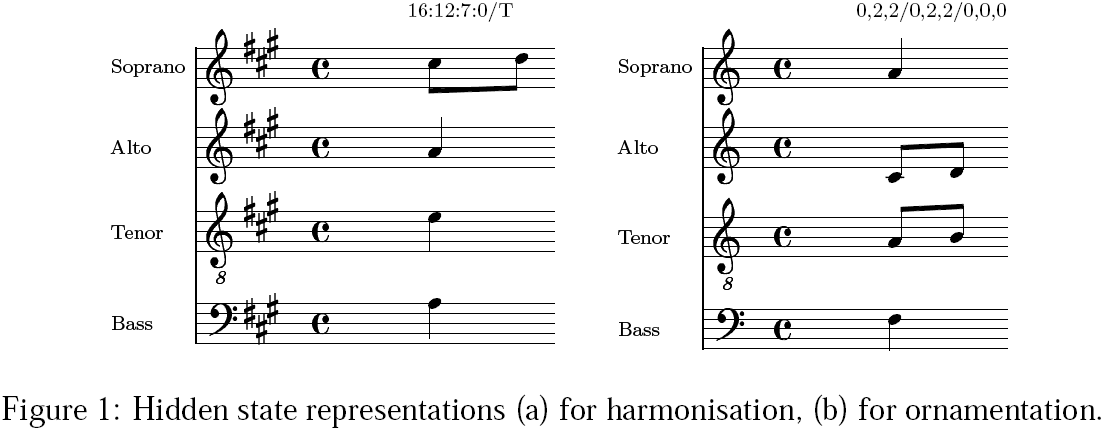
\includegraphics[width=8cm]{allan}}

}

%%%%%%%%%%%%%%%%%%%%%%%%%%%%%%%%%%%%%%%%%%%%%%%%%%%%%%%%%%%%%%%%%%%%%%%%%%%%%%%%

\slide{HMM example: Learning Bach}{

\item results: \url{http://www.anc.inf.ed.ac.uk/demos/hmmbach/}

~

\centerline{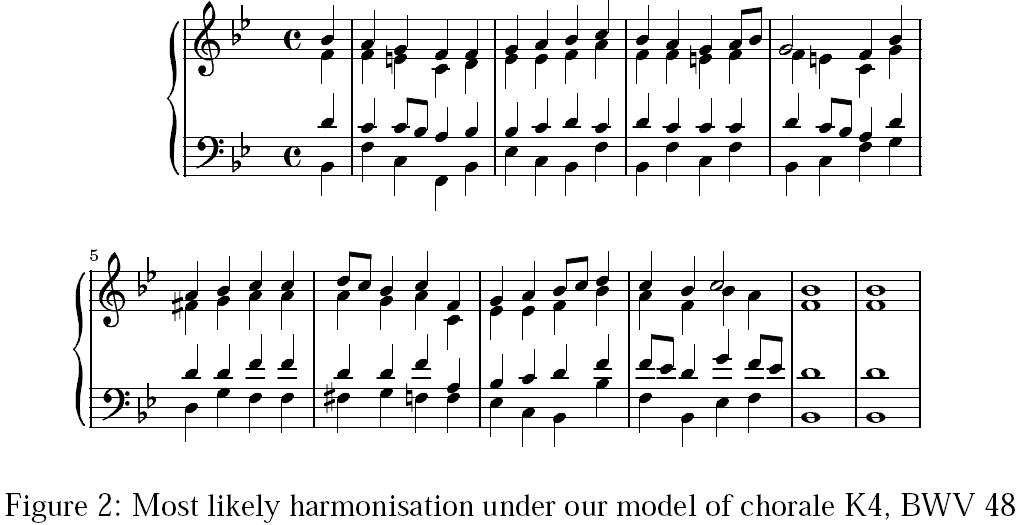
\includegraphics[width=8cm]{allan2}}

~

\item See also work by Gerhard
Widmer \url{http://www.cp.jku.at/people/widmer/}

}

%%%%%%%%%%%%%%%%%%%%%%%%%%%%%%%%%%%%%%%%%%%%%%%%%%%%%%%%%%%%%%%%%%%%%%%%%%%%%%%%

\key{Free energy formulation of EM}
\slide{Free Energy formulation of EM}{

~

\item We introduced EM rather heuristically: an iteration to resolve
the chicken and egg problem.

Are there convergence proofs?

Are there generalizations?

Are there more theoretical insights?

~

$\to$ Free Energy formulation of Expectation Maximization

}

%%%%%%%%%%%%%%%%%%%%%%%%%%%%%%%%%%%%%%%%%%%%%%%%%%%%%%%%%%%%%%%%%%%%%%%%%%%%%%%%

\slide{Free Energy formulation of EM}{

\item Define a function (called ``Free Energy'')
\begin{align*}
F(q,\t)
 &= \log P(Y ; \t) - \kld{q(X)}{P(X | Y;\t)}
\end{align*}
where{\small
\begin{align*}
&\log P(Y ; \t)
 = \log \sum_X P(X,Y; \t) \qquad \text{ log-likelihood of \emph{observed} data $Y$} \\
&\kld{q(X)}{P(X | Y;\t)}
 := \sum_X q(X) \log \frac{q(X)}{P(X \| Y;\t)} \quad \text{Kullback-Leibler div.}
\end{align*}
}
~

\item The Kullback-Leibler divergence is sort-of a distance measure between two
distributions: $\kld{q}{p}$ is always positive and zero only if $q=p$.

}

%%%%%%%%%%%%%%%%%%%%%%%%%%%%%%%%%%%%%%%%%%%%%%%%%%%%%%%%%%%%%%%%%%%%%%%%%%%%%%%%

\slide{Free Energy formulation of EM}{

\item We can write the free energy in two ways
{\small\begin{align}
F(q,\t)
 &= {\color{red}\underbrace{\log P(Y ; \t)}_{\text{data log-like.}}}
  - {\color{blue}\underbrace{\kld{q(X)}{P(X | Y;\t)}}_{\text{E-step:
 $q\gets\argmin$}}} \label{F1}\\
 &= \log P(Y ; \t) - \sum_X q(X) \log \frac{q(X)}{P(X \| Y;\t)} \nonumber\\
 &= \sum_X q(X) \log P(Y ; \t)
  + \sum_X q(X) \log P(X \| Y;\t)
  + H(q) \nonumber\\
 &= {\color{green}\underbrace{\sum_X q(X) \log
 P(X,Y;\t)}_{\text{M-step: $\t\gets\argmax$}}} + H(q), \label{F2}
\end{align}}

\mypause

\item We actually want to maximize {\color{red}$P(Y;\t)$} w.r.t.\ $\t$  $\to$ but
can't analytically

\item Instead, we maximize the lower bound $F(q,\t) \le \log P(Y;\t)$

-- {\color{blue} E-step:~ find $q$ that maximizes $F(q,\t)$ for fixed $\t^\old$
   using (\ref{F1})}

~~ ($\to$  $q(X)$ approximates $P(X | Y;\t)$, makes lower bound tight)

-- {\color{green}M-step:~ find $\t$ that maximizes $F(q,\t)$ for fixed $q$ using
   (\ref{F2})}

~~ ($\to$ $\t$ maximizes $Q(\t,q) = \sum_X q(X) \log P(X,Y;\t)$)

%\mypause

\item \textbf{Convergence proof:} $F(q,\t)$ increases in each step.

}

%%%%%%%%%%%%%%%%%%%%%%%%%%%%%%%%%%%%%%%%%%%%%%%%%%%%%%%%%%%%%%%%%%%%%%%%%%%%%%%%

\slide{}{

\item The free energy formulation of EM

-- clarifies convergence of EM (to \emph{local minima})

-- clarifies that $q$ need only to \emph{approximate} the posterior

~\mypause

\item \emph{Why is it called free energy?}

\mypause

\medskip

-- Given a physical system in specific state $(x,y)$, it has energy
   $E(x,y)$

~~ {\tiny This implies a joint distribution $p(x,z) = \frac{1}{Z}
e^{-E(x,y)}$ with partition function $Z$}

\medskip

-- If the DoFs $y$ are ``constrained'' and $x$ ``unconstrained'',

~~ then the \emph{expected energy} is $\<E\> = \sum_x q(x) E(x,y)$

~~ {\tiny Note $\<E\> = -Q(\t,q)$ is the same as the neg. expected
data log-likelihood}

\medskip

-- The unconstrained DoFs $x$ have an entropy $H(q)$

\medskip

-- Physicists call $A = \<E\> - H$ ~ (Helmholtz) free energy

~~ {\tiny Which is the negative of our eq.\ (\ref{F2}): $F(q,\t) = Q(\t,q) + H(q)$}

}

%%%%%%%%%%%%%%%%%%%%%%%%%%%%%%%%%%%%%%%%%%%%%%%%%%%%%%%%%%%%%%%%%%%%%%%%%%%%%%%%

\slide{Conditional vs.\ generative models}{

(very briefly)

}

%%%%%%%%%%%%%%%%%%%%%%%%%%%%%%%%%%%%%%%%%%%%%%%%%%%%%%%%%%%%%%%%%%%%%%%%%%%%%%%%

\key{Maximum conditional likelihood}
\slide{Maximum conditional likelihood}{

\item We have two random variables $X$ and $Y$ and full data $D=\{(x_i,y_i)\}$

Given a model $P(X,Y;\t)$ of the joint distribution we can train it
$$\t^\text{ML} = \argmax_\t \prod_i P(x_i,y_i;\t)$$

~

\item Assume the \emph{actual goal} is to have a classifier $x \mapsto
y$, or, the \emph{conditional} distribution $P(Y|X)$.

~

\emph{Q: Is it really necessary to first learn the full joint model
$P(X,Y)$ when we only need $P(Y|X)$?}

~

\emph{Q: If $P(X)$ is very complicated but $P(Y|X)$ easy, then
learning the joint $P(X,Y)$ is unnecessarily hard?}

}

%%%%%%%%%%%%%%%%%%%%%%%%%%%%%%%%%%%%%%%%%%%%%%%%%%%%%%%%%%%%%%%%%%%%%%%%%%%%%%%%

\slide{Maximum conditional Likelihood}{

Instead of likelihood maximization $\t^\text{ML} = \argmax_\t \prod_i P(x_i,y_i;\t)$:

~

\item \textbf{Maximum conditional likelihood:}

Given a \emph{conditional model} $P(Y|X;\t)$, train
$$\t^* = \argmax_\t \prod_i P(y_i | x_i;\t)$$

~

\item The little but essential difference: We don't care to learn
$P(X)$!

}

%%%%%%%%%%%%%%%%%%%%%%%%%%%%%%%%%%%%%%%%%%%%%%%%%%%%%%%%%%%%%%%%%%%%%%%%%%%%%%%%

\key{Conditional random field}
\slide{Example: Conditional Random Field}{\label{lastpage}

$$f(y,x) = \phi(y,x)^\T \b \quad = \sum_{j=1}^k \phi_j(y_{\del j},x) \b_j$$

$$p(y | x) = e^{f(y,x) - Z(x,\b)} \quad \propto \prod_{j=1}^k e^{\phi_j(y_{\del j},x) \b_j}$$


~

\item Logistic regression also maximizes the
conditional log-likelihood

\item Plain regression also maximizes the
conditional log-likelihood! (with $\log P(y_i|x_i;\b) \propto (y_i
- \phi(x_i)^\T\b)^2$)

}

%%%%%%%%%%%%%%%%%%%%%%%%%%%%%%%%%%%%%%%%%%%%%%%%%%%%%%%%%%%%%%%%%%%%%%%%%%%%%%%%

\slidesfoot

%%%%%%%%%%%%%%%%%%%%%%%%%%%%%%%%%%%%%%%%%%%%%%%%%%%%%%%%%%%%%%%%%%%%%%%%%%%%%%%%

%% \slide{Belief Propagation remarks}{

%% \item Belief Propagation is also called \textbf{Sum-Product
%% algorithm} or \textbf{Message passing}.

%% ~

%% \item When replacing all $\sum$ by $\max$ in the BP equations, then we
%% get the so-called \textbf{Max-Product algorithm}

%% -- Max-Product does not compute marginal probabilities $P(X_i)$ but
%%    the global MAP $\argmax_{X_{1:n}} P(X_{1:n})$, that is, the most
%%    likely of all global configurations of all random variables.


%% ~

%% \item When computing in the log-domain, that is, compute log-messages
%%    $\log \mu$ instead of messages, the Max-Product algorithm becomes
%%    a \textbf{Max-Sum algorithm}

%% }

%% %%%%%%%%%%%%%%%%%%%%%%%%%%%%%%%%%%%%%%%%%%%%%%%%%%%%%%%%%%%%%%%%%%%%%%%%%%%%%%%%

%% \slide{example}{

%% \centerline{\input{figs/vl2-asia}}

%% -- eliminate in order $D,B,S,L,A,T,X,E$

%% -- eliminate in order $E,$... (not good)

%% -- eliminate in order $D,X,A,S,B,L,T,E$

%% ~

%% \item on the Junction Tree, we can use BP (the special case
%%    factor-to-factor message equations) to do exact inference.


%% }

%%%%%%%%%%%%%%%%%%%%%%%%%%%%%%%%%%%%%%%%%%%%%%%%%%%%%%%%%%%%%%%%%%%%%%%%%%%%%%%%

%% \slide{Variable Elimination example}{

%% ~

%% \shows[.7]{vl3-Jordan-BNet}
%% $$
%% P(x_{1:6})
%%  = P(x_1)~ P(x_2|x_1)~ P(x_3|x_1)~ P(x_4|x_2)~ P(x_5|x_3)~ P(x_6|x_2,x_5)
%% $$

%% ~

%% problem: compute $P(x_5)$

%% %% {\tiny

%% %% In the exercises: compute $P(x_1,x_6)$

%% %% }

%% }

%%%%%%%%%%%%%%%%%%%%%%%%%%%%%%%%%%%%%%%%%%%%%%%%%%%%%%%%%%%%%%%%%%%%%%%%%%%%%%%%


%% %%%%%%%%%%%%%%%%%%%%%%%%%%%%%%%%%%%%%%%%%%%%%%%%%%%%%%%%%%%%%%%%%%%%%%%%%%%%%%%%

%% \slide{digression: additive decomposable functions}{

%% \small

%% \item graphical models describe how a joint factors

%% -- factorization corresponds to independence (by def)

%% -- factors correspond to ``directly coupled/interacting'' variables

%% ~

%% \item take the neg-log of the joint:
%% \begin{align*}
%% E(X_{1:n})
%%  &:= -\log P(X_{1:n}) = \sum_{i=1}^k \phi_i(X_{C_i})
%%  \quad\text{with}\quad \phi_i =-\log f_i
%% \end{align*}
%% assigns an \emph{error} or \emph{energy} to every possible
%% configuration $x_{1:n}$

%% [Physics: at temperature $T$ an ensemble of particles is distributed as
%% $P(X_{1:n})\propto \exp(-E(X_{1:n})/T)$]

%% ~

%% \item $E(X_{1:n})$ is an additive decomposable function!

%% -- optimization: find $\argmin_{X_{1:n}} E(X_{1:n})$ 

%% -- additive decomposition makes optimization easier

%% -- expresses independence in the sense of optimization

%% -- optimization of $E$ closely related to inference in $P$

%% }

